%%%%%%%%%%%%%%%%%%%%%%%%%%%%%%%%%%%%%%%%%%%%%%%%%%%%%%%%%%%%%%%%%%%%%%
% Overleaf (WriteLaTeX) Example: Molecular Chemistry Presentation
%
% Source: http://www.overleaf.com
%
% In these slides we show how Overleaf can be used with standard 
% chemistry packages to easily create professional presentations.
% 
% Feel free to distribute this example, but please keep the referral
% to overleaf.com
% 
%%%%%%%%%%%%%%%%%%%%%%%%%%%%%%%%%%%%%%%%%%%%%%%%%%%%%%%%%%%%%%%%%%%%%%

\documentclass[xcolor={dvipsnames}]{beamer}

\mode<presentation>
{
  \usetheme{Madrid}       % or try default, Darmstadt, Warsaw, ...
  \usecolortheme{default} % or try albatross, beaver, crane, ...
  \usefonttheme{default}    % or try default, structurebold, ...
  \setbeamertemplate{navigation symbols}{}
  \setbeamertemplate{caption}[numbered]
} 

\usepackage[english]{babel}
\usepackage[utf8x]{inputenc}
\usepackage{graphicx}
\usepackage{hyperref}
  \hypersetup{colorlinks=true}
  \hypersetup{urlcolor=blue}
  \hypersetup{linkcolor = .}
\usepackage{xcolor}
\usepackage{siunitx}
  \sisetup{separate-uncertainty = true}
\usepackage{physics}
\usepackage[font=small,labelfont=bf]{caption}
\usepackage{subcaption}
\usepackage[en-GB]{datetime2}
\usepackage{overpic}
\usepackage{feynmp}
\DeclareGraphicsRule{*}{mps}{*}{}
\usepackage{scalerel}
\newcommand{\mylbrace}[2]{\vspace{#2pt}\hspace{6pt}\scaleleftright[\dimexpr5pt+#1\dimexpr0.06pt]{\lbrace}{\rule[\dimexpr2pt-#1\dimexpr0.5pt]{-4pt}{#1pt}}{.}}
\newcommand{\myrbrace}[2]{\vspace{#2pt}\scaleleftright[\dimexpr5pt+#1\dimexpr0.06pt]{.}{\rule[\dimexpr2pt-#1\dimexpr0.5pt]{-4pt}{#1pt}}{\rbrace}\hspace{6pt}}

% Trim in percent
\usepackage{adjustbox}

% No "Figure" prefix
\setbeamertemplate{caption}{\raggedright\insertcaption\par}

% Nice decay amplitude diagrams
\usepackage{amsmath,amssymb,tikz-cd}

% Strike out text
\usepackage[normalem]{ulem}

% For figures with text overlay
\usepackage{overpic}

% Arrows
\usepackage{tikz}
\newcommand{\tikzmark}[1]{\tikz[remember picture] \node[coordinate] (#1) {#1};}

% Colourbox with line breaks
\newcommand{\cbox}[2][lime!20]{%
  \colorbox{#1}{\parbox{\dimexpr\linewidth-2\fboxsep}{\strut #2\strut}}%
}

% Vector arrows
\usepackage[pdftex]{pict2e}

% Checkmark symbol
\def\checkmark{\tikz\fill[scale=0.4](0,.35) -- (.25,0) -- (1,.7) -- (.25,.15) -- cycle;} 

% Here's where the presentation starts, with the info for the title slide
\title[LHCb-UK RAL]{Update of $\gamma$ in $B^\pm\to[K^+K^-\pi^+\pi^-]_Dh^\pm$ with external strong-phase inputs}

\author[Martin Tat]{Martin Tat}
\institute[University of Oxford]{\normalsize University of Oxford\\ \vspace{0.3cm}\normalsize LHCb-UK annual meeting, RAL}
\date{8th-10th January 2024}

\titlegraphic{
\includegraphics[height = 2.3cm]{lhcb.jpg}\hspace{1.5cm}~%
              
\includegraphics[height = 2.3cm]{OxfordLogo.pdf}}

\begin{document}

\begin{frame}
  \titlepage
\end{frame}

% These three lines create an automatically generated table of contents.
% \begin{frame}{Outline}
%   \tableofcontents
% \end{frame}

\section{Introduction to \texorpdfstring{$\gamma$}{gamma} and \texorpdfstring{$C\!P$}{CP} violation}
\begin{frame}{Introduction to $\gamma$ and $C\!P$ violation}
  \begin{itemize}
    \setlength\itemsep{0.3em}
    \item{CPV in SM is described by the Unitary Triangle, with angles $\alpha$, $\beta$, $\gamma$}
    \item{The angle $\gamma = \text{arg}\Big(-\frac{V^{\phantom{*}}_{ud}V^*_{ub}}{V^{\phantom{*}}_{cd}V^*_{cb}}\Big)$ is very important:}
    \begin{enumerate}
    \setlength\itemsep{0.2em}
      \item{Negligible theoretical uncertainties: Ideal SM benchmark}
      \item{Accessible at tree level: Indirectly probe New Physics that enter loops}
      \item{Compare with a global CKM fit: Is the Unitary Triangle a triangle?}
    \end{enumerate}
  \end{itemize}
  \vspace{-0.2cm}
  \begin{figure}
    \centering
    \begin{subfigure}{0.5\textwidth}
      \centering
      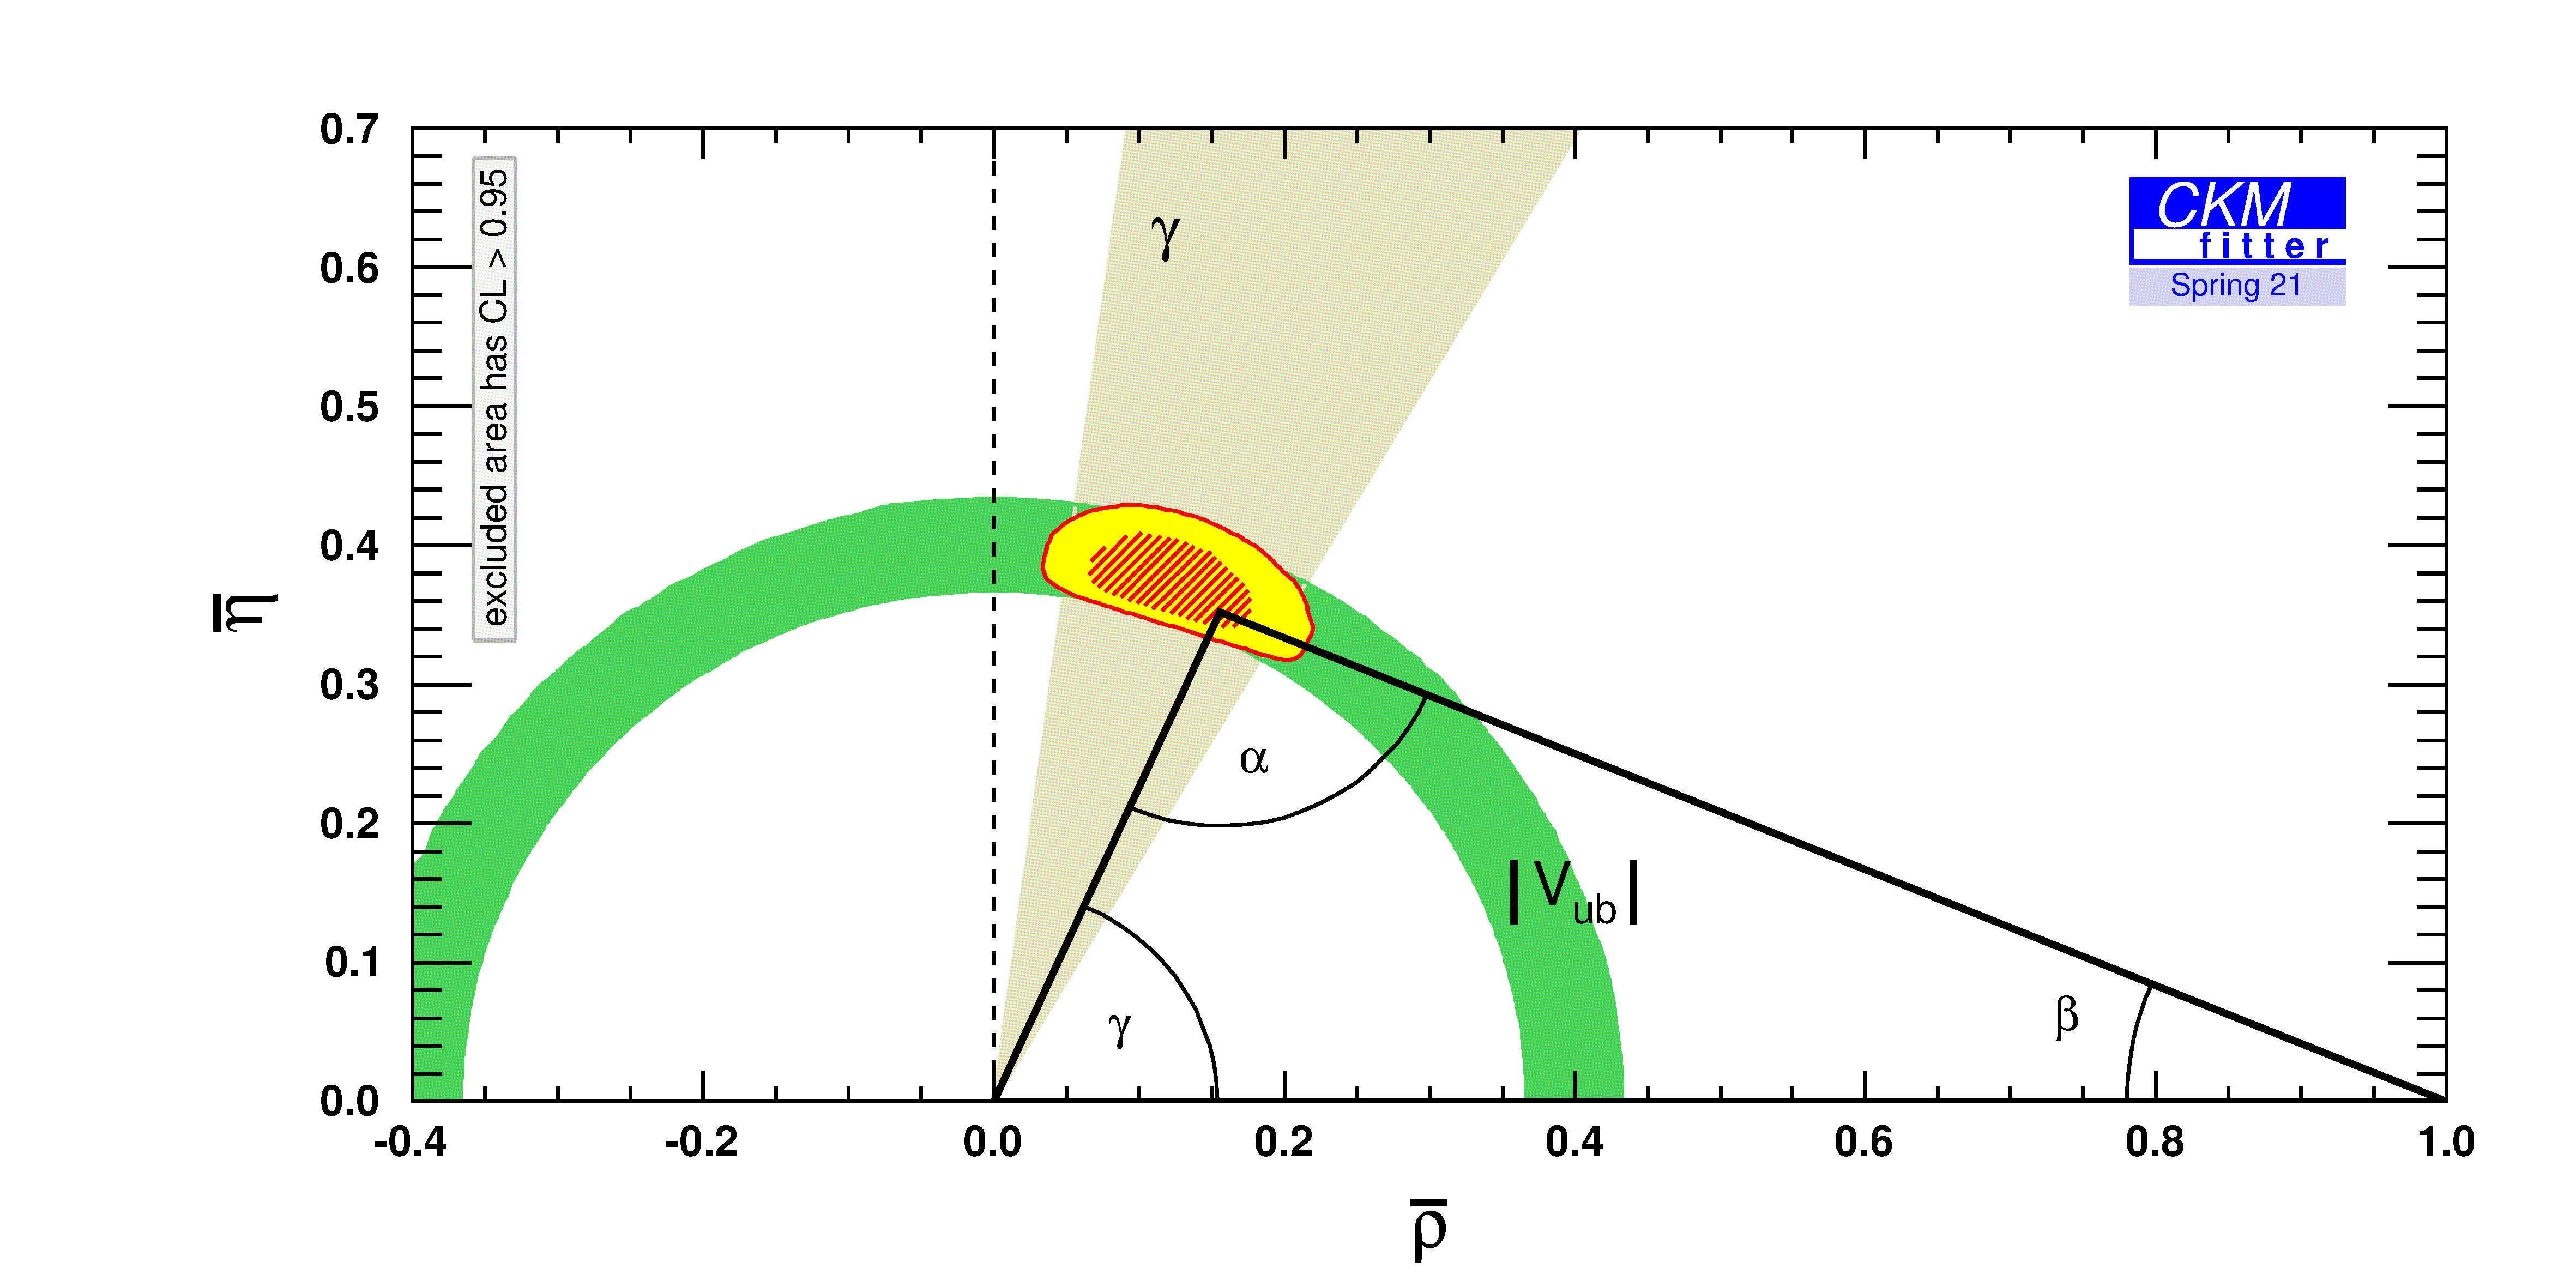
\includegraphics[width = 1.0\textwidth]{Plots/ckmfitter_tree.png}
      \caption{Tree level: $\gamma = \big(72.1^{+5.4}_{-5.7}\big)^\circ$}
    \end{subfigure}%
    \begin{subfigure}{0.5\textwidth}
      \centering
      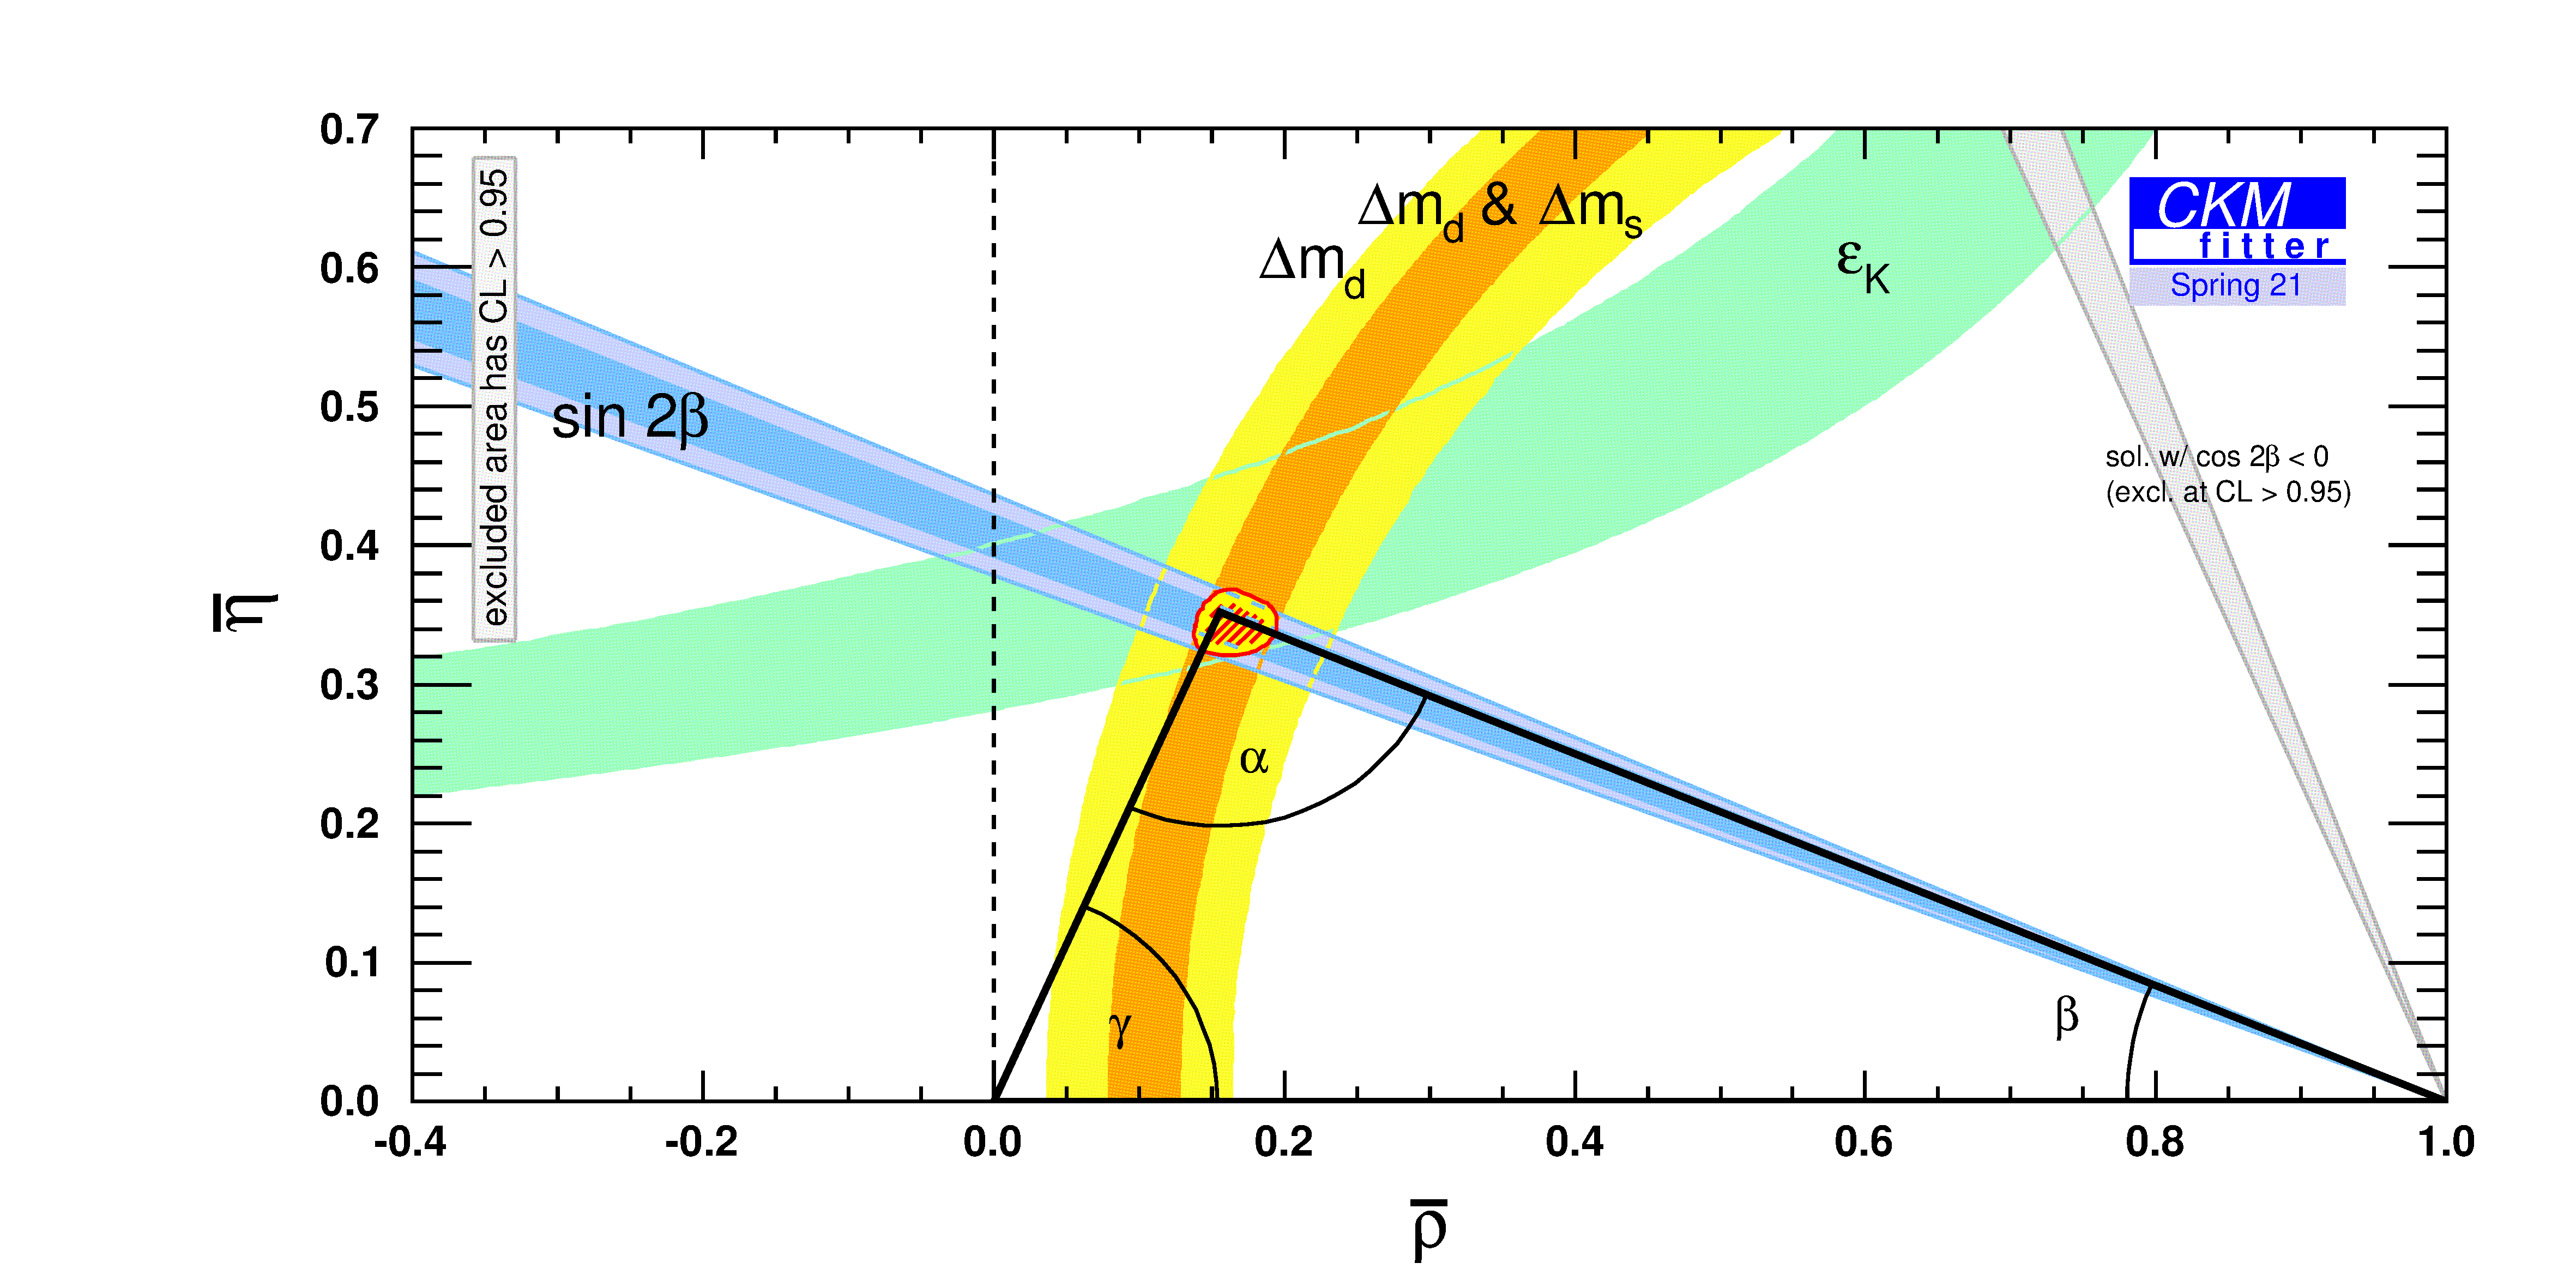
\includegraphics[width = 1.0\textwidth]{Plots/ckmfitter_loop.png}
      \caption{Loop level: $\gamma = \big(65.5^{+1.1}_{-2.7}\big)^\circ$}
    \end{subfigure}
    \vspace{-0.3cm}
    \captionsetup{justification=centering}
    \caption*{\centering\tiny CKMfitter Group (J. Charles et al.), Eur. Phys. J. C41, 1-131 (2005), updated results and plots available at: \href{http://ckmfitter.in2p3.fr}{http://ckmfitter.in2p3.fr}}
  \end{figure}
\end{frame}

\begin{frame}{Sensitivity through interference}
  \begin{center}
    \Large Measure $\gamma$ through interference effects in $B^\pm\to DK^\pm$
  \end{center}
  \begin{figure}[H]
    \centering
    \begin{subfigure}{0.5\textwidth}
      \centering
      \begin{fmffile}{fgraph/fgraph_BtoDK1}
        \setlength{\unitlength}{0.4cm}
        \begin{fmfgraph*}(6,6)
          \fmfstraight
          \fmfleft{i1,B,i2,t1,t2,t3,t9,t10}
          \fmfright{o1,D,o2,t4,t5,o3,K,o4}
          \fmflabel{$\bar{u}$}{i1}
          \fmflabel{$b$}{i2}
          \fmfv{l.d=20,l.a=180,l={$B^-$\mylbrace{30}{-8}}}{B}
          \fmflabel{$\bar{u}$}{o1}
          \fmflabel{$c$}{o2}
          \fmflabel{$\bar{u}$}{o3}
          \fmflabel{$s$}{o4}
          \fmfv{l.d=15,l.a=0,l={\myrbrace{30}{-12}}$D^0$}{D}
          \fmfv{l.d=15,l.a=0,l={\myrbrace{30}{11}}$K^-$}{K}
          \fmf{fermion}{o1,i1}
          \fmf{fermion,tension=1.5}{i2,v1}
          \fmf{fermion}{v1,o2}
          \fmf{phantom,tension=1.5}{t9,v2}
          \fmf{boson,label=$W$,label.side=left,tension=0}{v1,v2}
          \fmf{fermion}{v2,o4}
          \fmf{fermion}{o3,v2}
        \end{fmfgraph*}
      \end{fmffile}
      \vspace{0.5cm}
      \caption*{Favoured $B^-\to D^0K^-$}
    \end{subfigure}%
    \begin{subfigure}{0.5\textwidth}
      \centering
      \begin{fmffile}{fgraph/fgraph_BtoDK2}
        \setlength{\unitlength}{0.4cm}
        \begin{fmfgraph*}(6,6)
          \fmfstraight
          \fmfleft{i1,t1,t2,B,t9,t10,i2}
          \fmfright{o1,K,o2,t4,t5,o3,D,o4}
          \fmflabel{$\bar{u}$}{i1}
          \fmflabel{$b$}{i2}
          \fmfv{l.d=20,l.a=180,l={$B^-$\mylbrace{100}{-8}}}{B}
          \fmflabel{$\bar{u}$}{o1}
          \fmflabel{$s$}{o2}
          \fmflabel{$\bar{c}$}{o3}
          \fmflabel{$u$}{o4}
          \fmfv{l.d=15,l.a=0,l={\myrbrace{30}{13}}$\bar{D^0}$}{D}
          \fmfv{l.d=15,l.a=0,l={\myrbrace{30}{-13}}$K^-$}{K}
          \fmf{fermion}{o1,i1}
          \fmf{fermion,tension=1.5}{i2,v1}
          \fmf{fermion}{v1,o4}
          \fmf{phantom,tension=1.5}{t2,v2}
          \fmf{boson,label=$W$,label.side=left,tension=0}{v1,v2}
          \fmf{fermion}{v2,o2}
          \fmf{fermion}{o3,v2}
        \end{fmfgraph*}
      \end{fmffile}
      \vspace{0.5cm}
      \caption*{Suppressed $B^-\to\bar{D^0}K^-$}
    \end{subfigure}
  \end{figure}
  \vspace{-0.3cm}
  \begin{itemize}
    \item{Superposition of $D^0$ and $\bar{D^0}$}
    \begin{itemize}
      \item{Consider $D^0$/$\bar{D^0}$ decays to the same final state, such as $D\to K^+K^-$}
    \end{itemize}
    \item{$b\to u\bar{c}s$ and $b\to c\bar{u}s$ interference $\to$ Sensitivity to $\gamma$}
  \end{itemize}
  \vspace{-0.3cm}
  \begin{center}
    $\mathcal{A}(B^-)=\mathcal{A}_B\Big(\mathcal{A}_{D^0} + r_Be^{i(\delta_B - \gamma)}\mathcal{A}_{\bar{D^0}}\Big)$ \\
    $\mathcal{A}(B^+)=\mathcal{A}_B\Big(\mathcal{A}_{\bar{D^0}} + r_Be^{i(\delta_B + \gamma)}\mathcal{A}_{D^0}\Big)$ \\
  \end{center}
\end{frame}

\begin{frame}[fragile]{Multi-body $D$ decays}
  \begin{center}
    This talk: Discuss $D\to K^+K^-\pi^+\pi^-$, where interference effects vary across phase space
  \end{center}
  \vspace{-0.3cm}
  \begin{itemize}
    \setlength\itemsep{0.5em}
    \item{Strong-phase difference $\delta_D$ is a function of phase space}
    \item{Compare yields of $B^+$ and $B^-$ and determine the asymmetry \underline{in local phase space regions}}
  \end{itemize}
  \begin{equation*}
    \begin{tikzcd}[column sep=huge]
      & D^0K^- \arrow[dr, bend left = 25, "\mathcal{A}_{D^0}(\Phi)"] & \\
      B^- \arrow[ur, bend left, "\mathcal{A}_B"] \arrow[dr, bend right, "\mathcal{A}_B r_B e^{i(\delta_B - \gamma)}"'] & [5cm] & DK^- \\
      & \bar{D^0}K^- \arrow[ur, bend right = 25, "\mathcal{A}_{\bar{D^0}}(\Phi)"'] & \\
    \end{tikzcd}
  \end{equation*}
  \vspace{-0.9cm}
  \begin{align*}
    \lvert\mathcal{A}(B^-)\lvert^2&\propto\lvert\mathcal{A}_{D^0}(\Phi)\lvert^2 + r_B^2\lvert\mathcal{A}_{\bar{D^0}}(\Phi)\lvert^2 \\
    &+ 2r_B\lvert\mathcal{A}_{D^0}(\Phi)\lvert\lvert\mathcal{A}_{\bar{D^0}}(\Phi)\lvert\cos(\delta_B - \gamma + \delta_D)
  \end{align*}
\end{frame}

\begin{frame}{Multi-body $D$ decays}
  \begin{itemize}
    \setlength\itemsep{0.5em}
    \item{Interpretation of $\gamma$ from the multi-body charm decays require external inputs of the charm strong-phase differences}
    \item{Measure model-independent strong-phases at a charm factory, such as BESIII, using an optimised binning scheme}
  \end{itemize}
  \begin{figure}
    \centering
    \begin{subfigure}{0.5\textwidth}
      \centering
      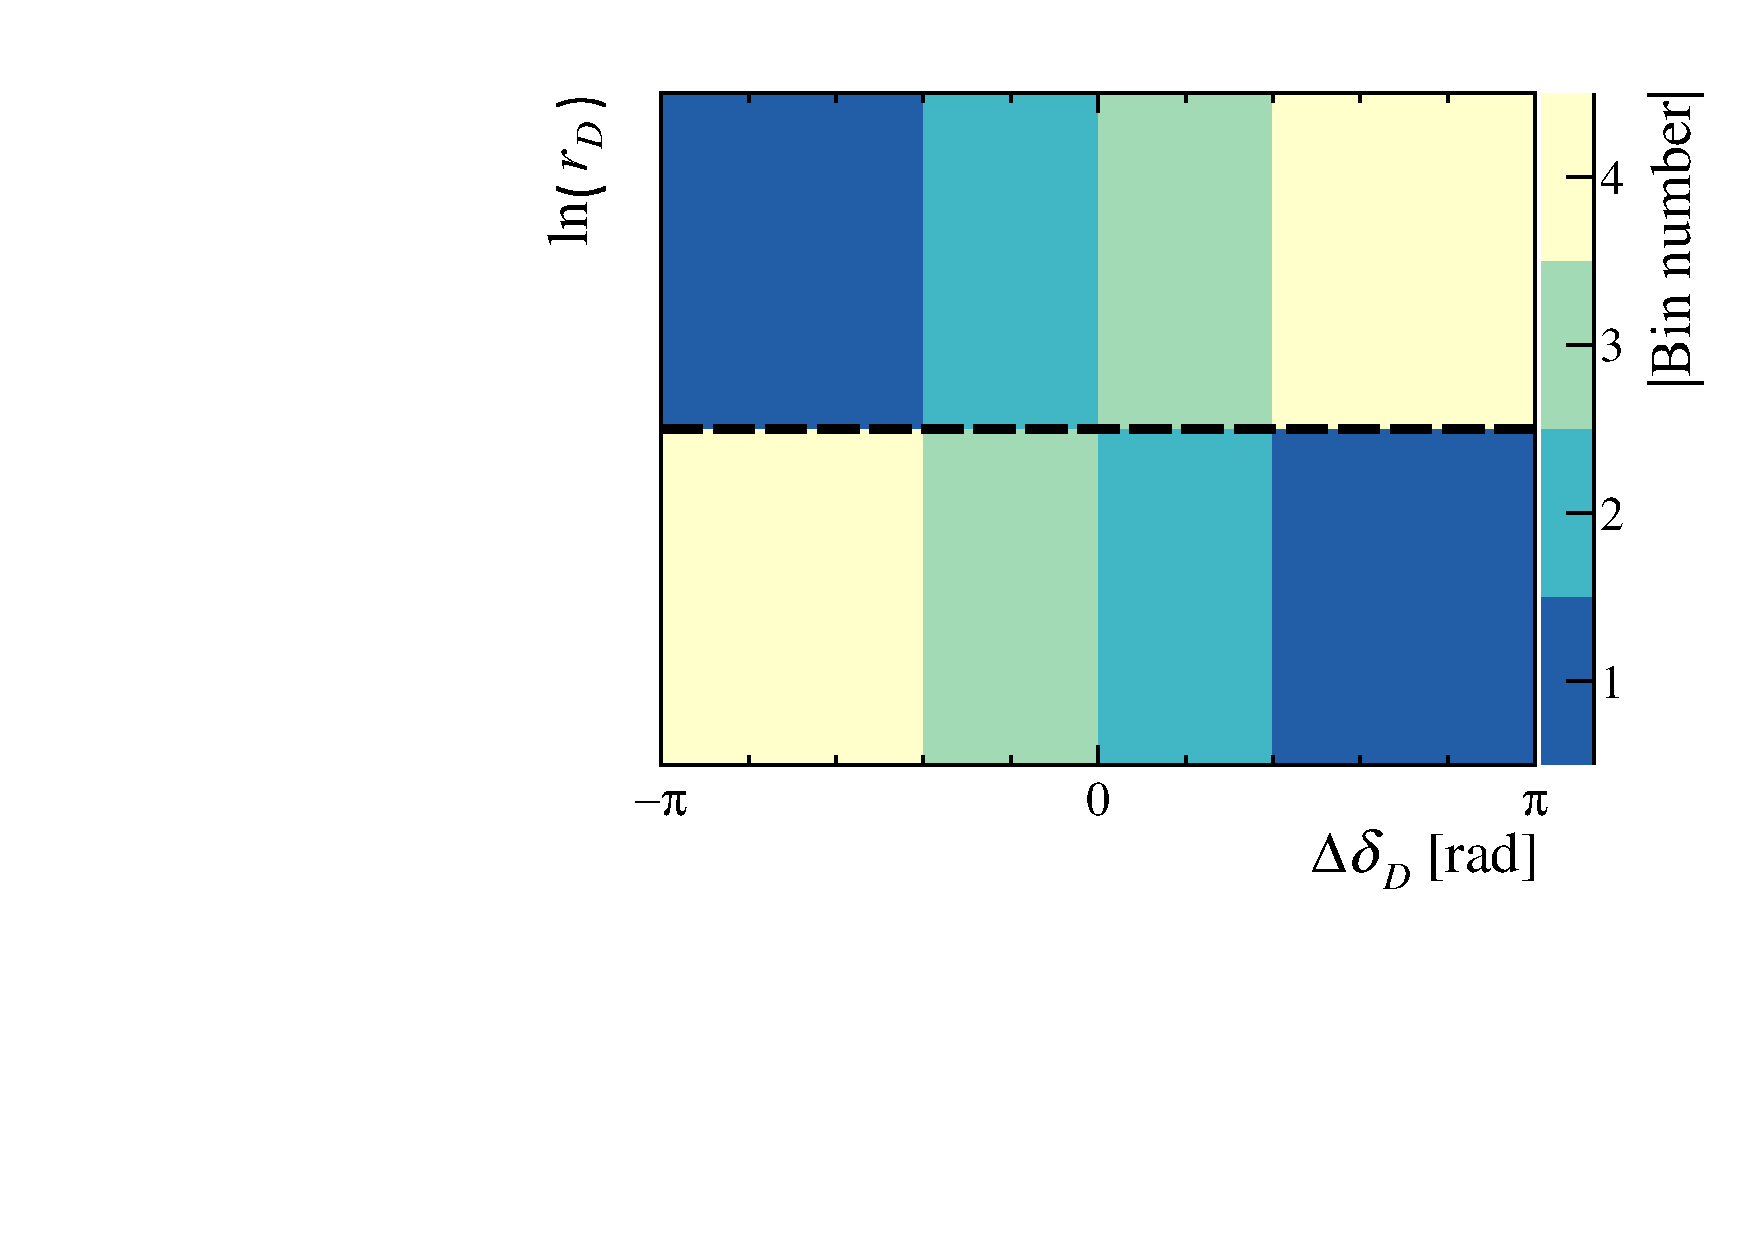
\includegraphics[height = 3.5cm]{Plots/BinningSchemePlot_4Bins.pdf}
      \vspace{-0.3cm}
      \caption*{4 bins}
    \end{subfigure}%
    \begin{subfigure}{0.5\textwidth}
      \centering
      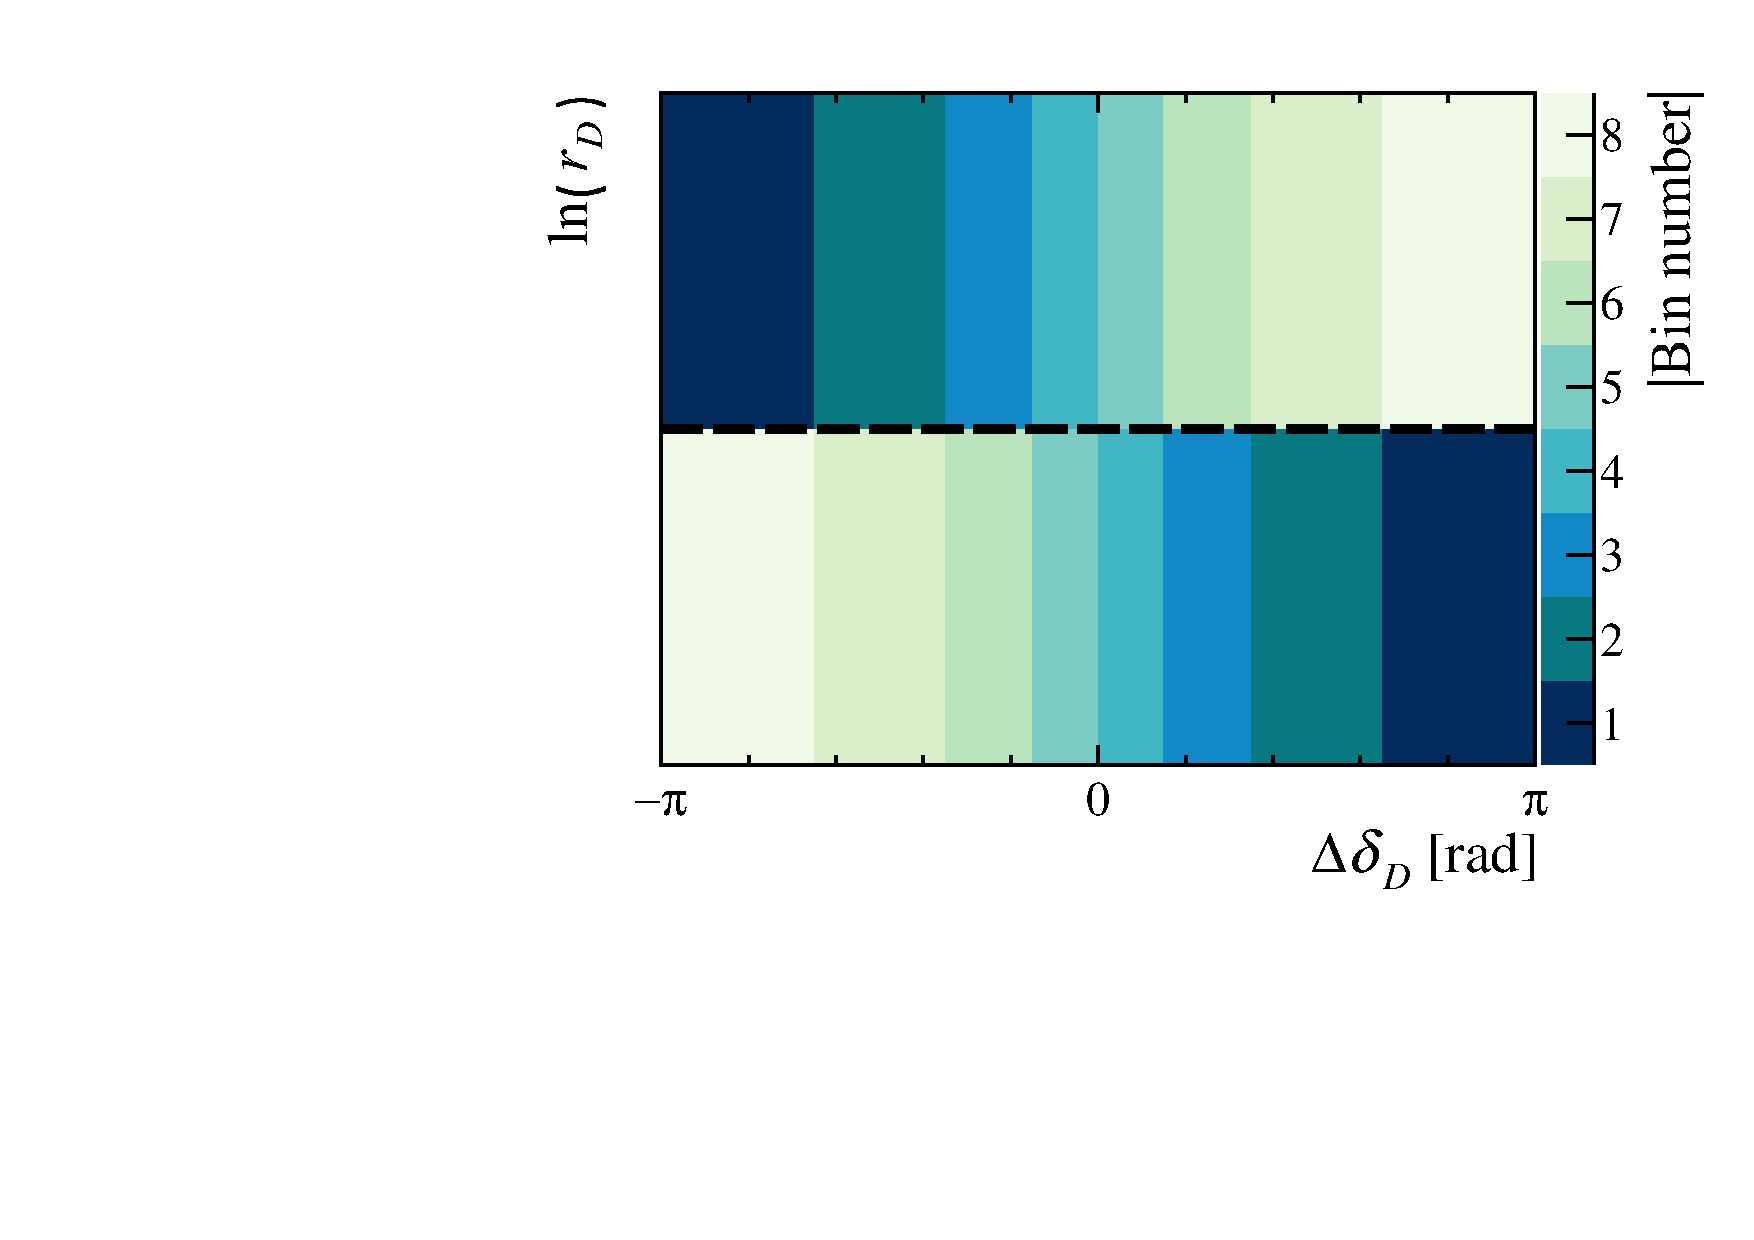
\includegraphics[height = 3.5cm]{Plots/BinningSchemePlot_8Bins.pdf}
      \vspace{-0.3cm}
      \caption*{8 bins}
    \end{subfigure}
    \caption*{\tiny\href{https://link.springer.com/article/10.1140/epjc/s10052-023-11560-5}{Eur. Phys. J. C \textbf{83}, 547 (2023)}}
  \end{figure}
\end{frame}

\begin{frame}{Phase-space binned $B^\pm\to[K^+K^-\pi^+\pi^-]_DK^\pm$}
  \begin{center}
    {\large Fully charged final state $\implies$ Highly suitable for LHCb}
  \end{center}
  \begin{figure}
    \centering
    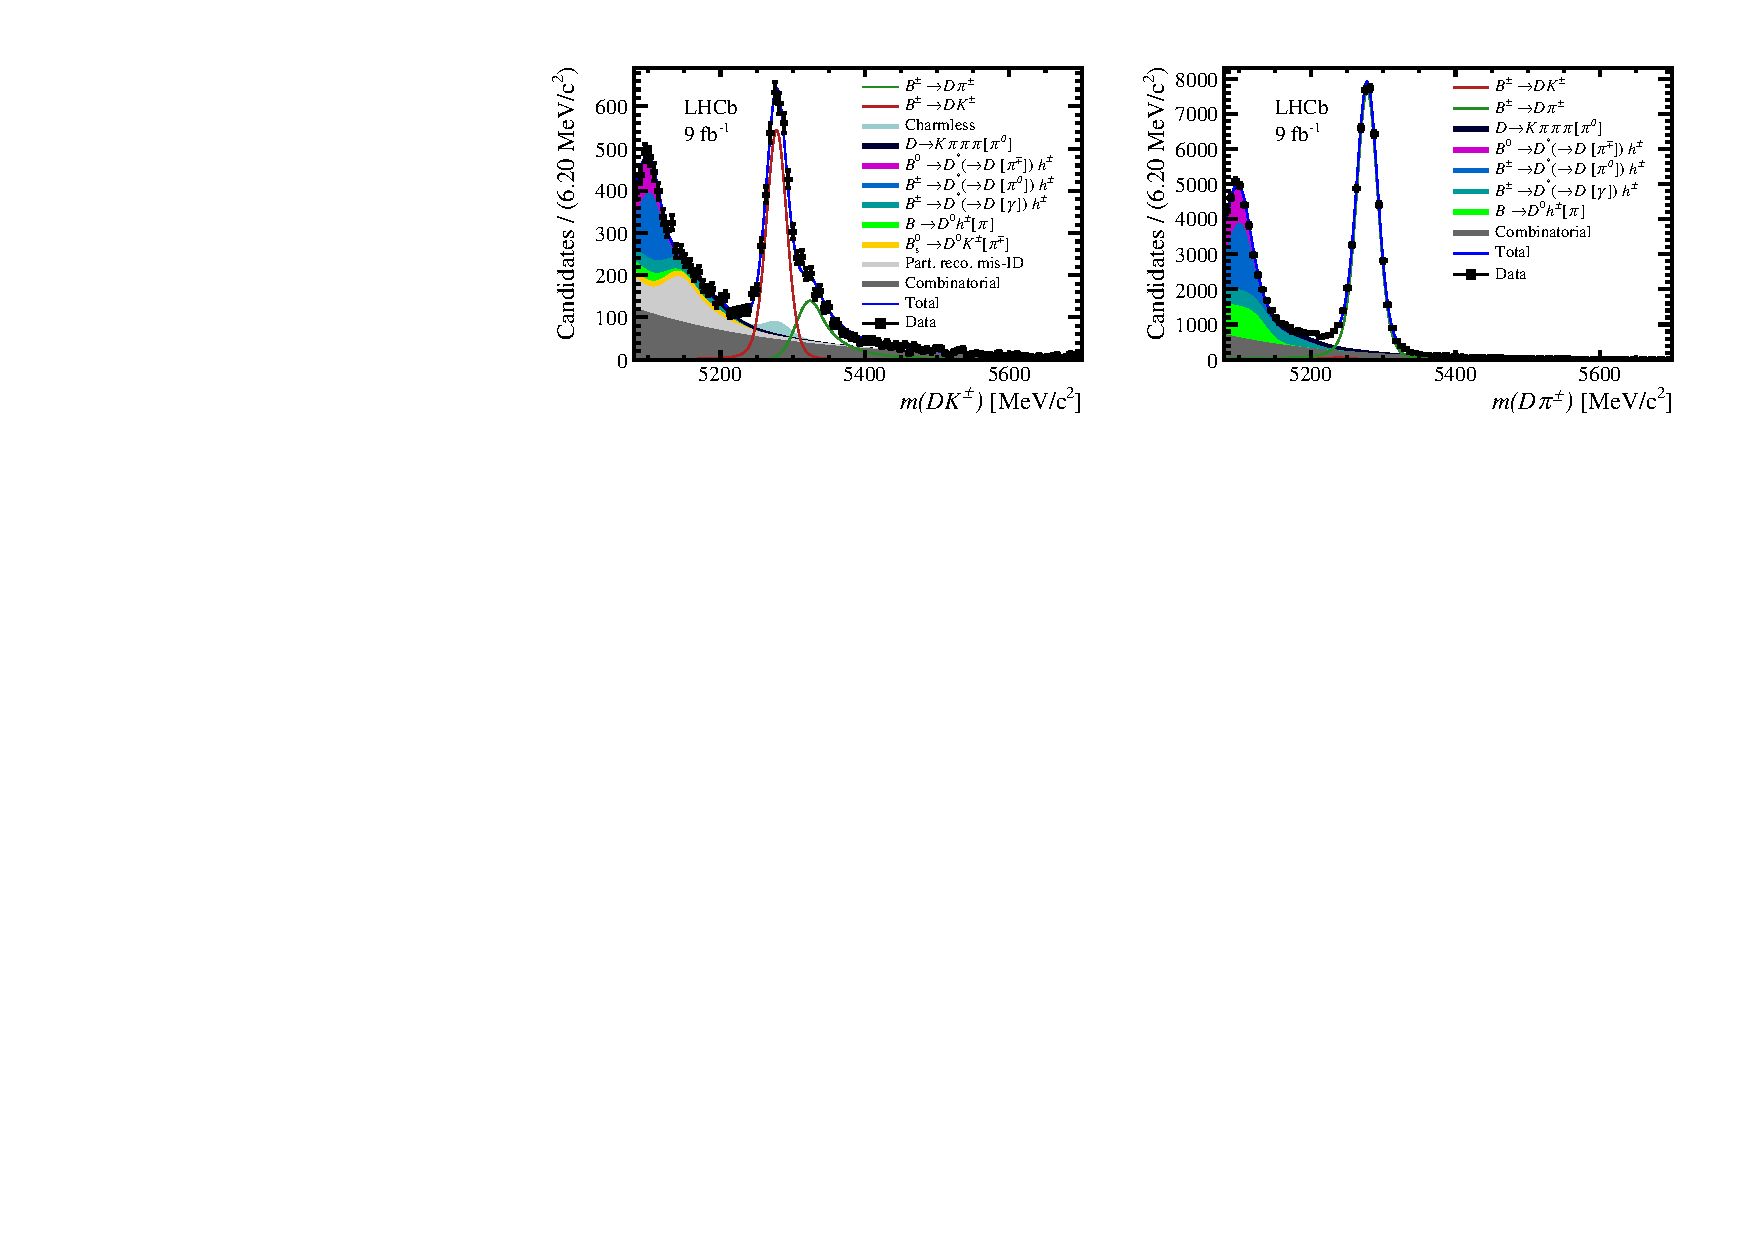
\includegraphics[width = 1.0\textwidth,trim={0 0 0 0},clip=true]{Plots/d2kkpipi_fiveL_allDP.pdf}
    \caption*{\tiny\href{https://link.springer.com/article/10.1140/epjc/s10052-023-11560-5}{Eur. Phys. J. C \textbf{83}, 547 (2023)}}
  \end{figure}
  \vspace{-0.5cm}
  \begin{itemize}
    \item{$B^\pm\to[K^+K^-\pi^+\pi^-]_Dh^\pm$ signal yield:}
    \begin{itemize}
      \item{$B^\pm\to DK^\pm$: $3026 \pm 38$}
      \item{$B^\pm\to D\pi^\pm$: $44349 \pm 218$}
    \end{itemize}
  \end{itemize}
\end{frame}

\begin{frame}{Phase-space binned $B^\pm\to[K^+K^-\pi^+\pi^-]_DK^\pm$}
  \begin{center}
    \large From the phase-space binned asymmetries, we obtain:\\
    \vspace{0.2cm}
    $\gamma = (116^{+12}_{-14})^\circ$
  \end{center}
  \vspace{-0.2cm}
  \begin{figure}[htb]
    \centering
    \begin{subfigure}{0.5\textwidth}
      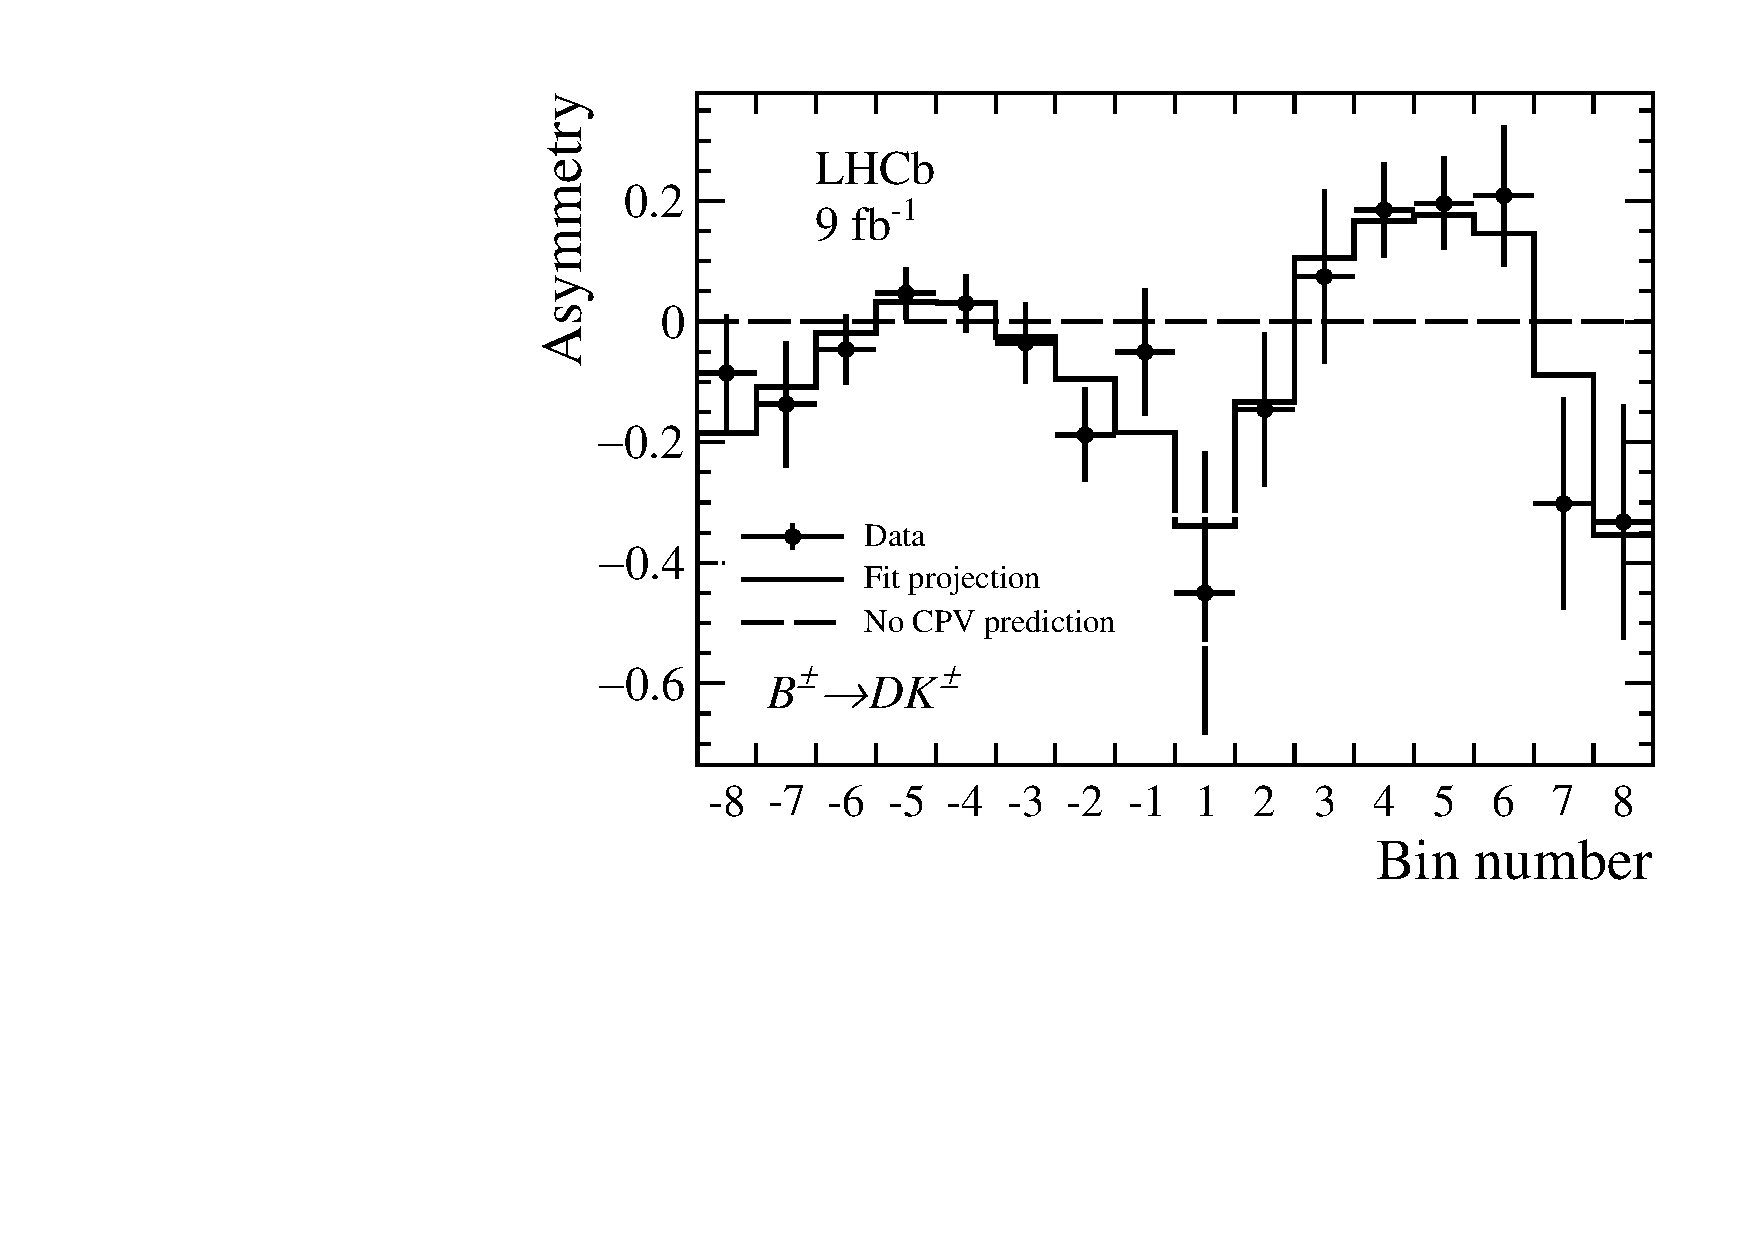
\includegraphics[width=1\textwidth]{Plots/BinAsymmetries_dk.pdf}
    \end{subfigure}%
    \begin{subfigure}{0.5\textwidth}
      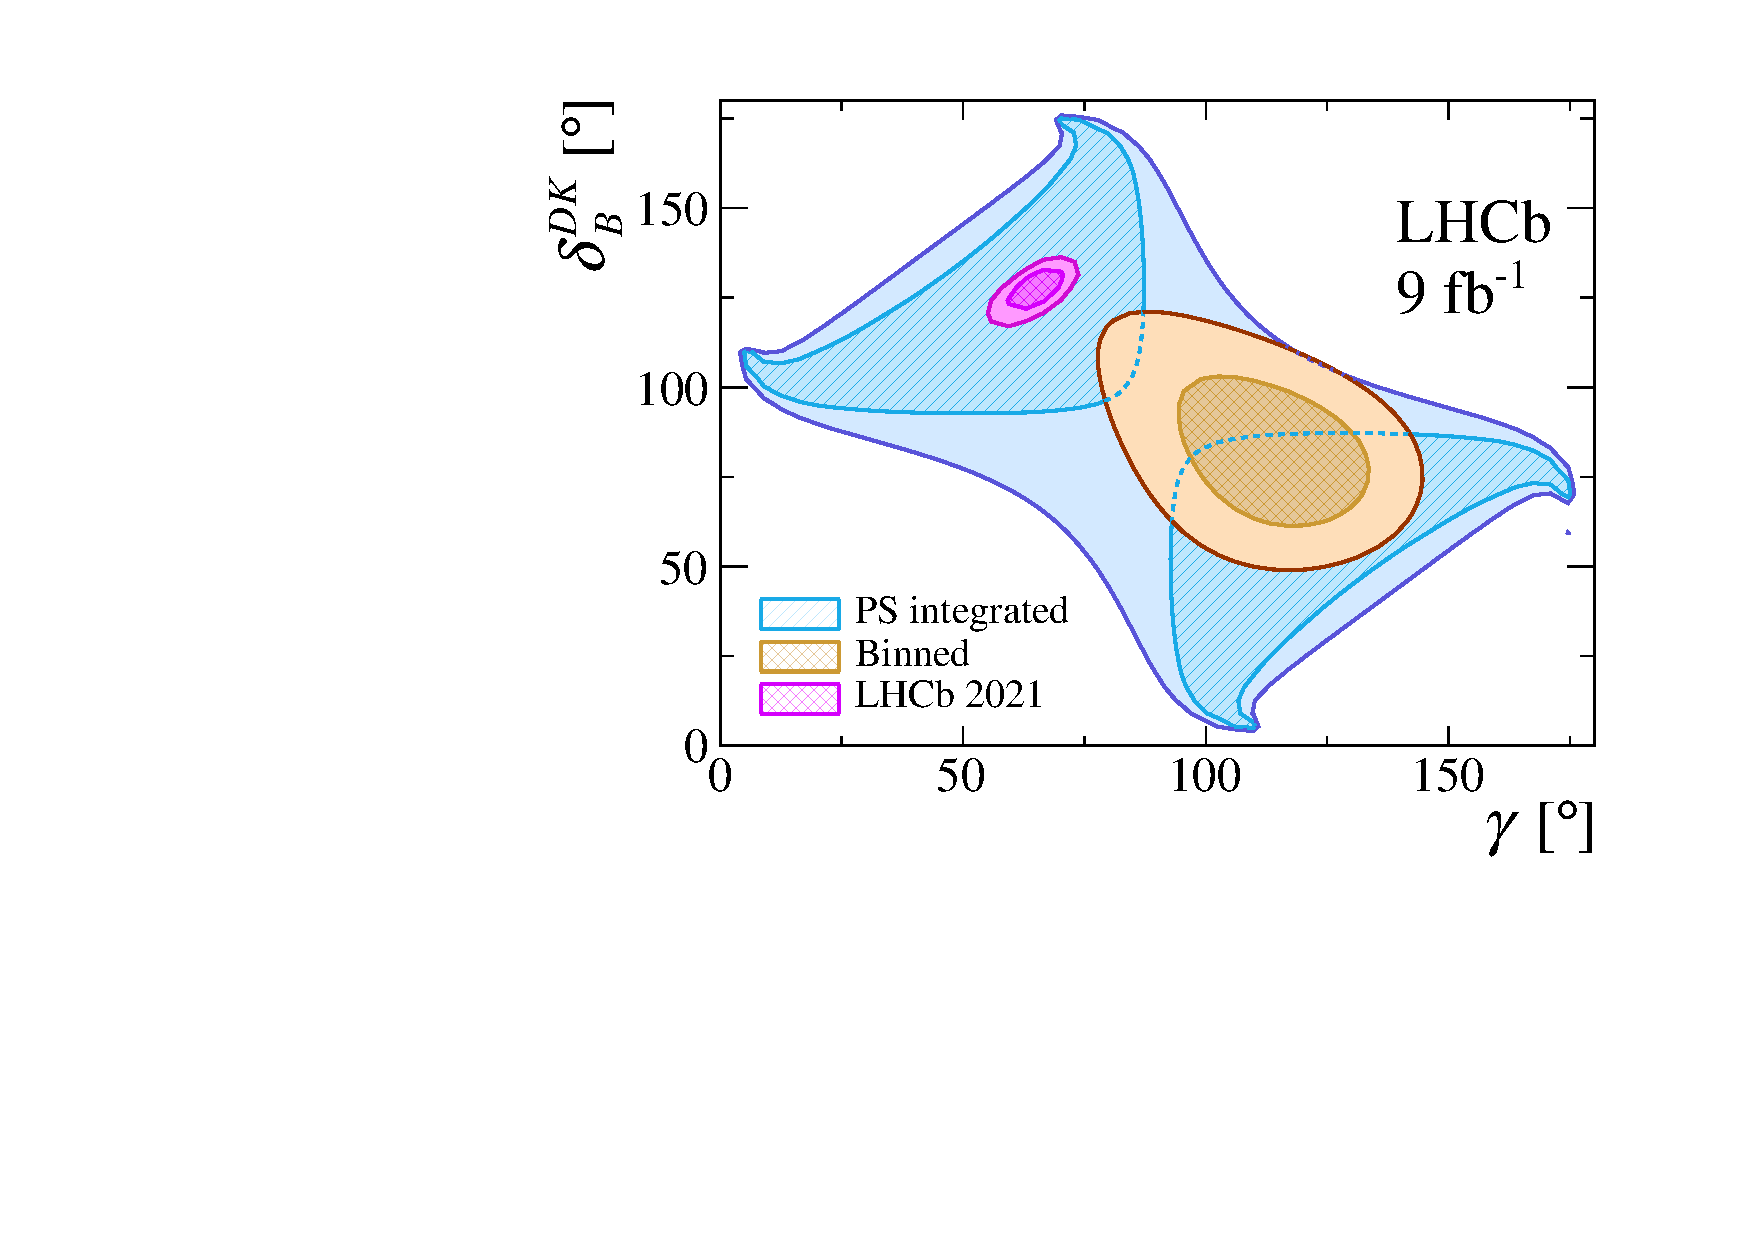
\includegraphics[width=1\textwidth]{Plots/gammacharm_lhcb_KKpipi_GLW_KKpipi_GGSZ_lhcb_2020_beauty_and_charm_g_d_dk.pdf}
    \end{subfigure}
    \vspace{-0.5cm}
    \caption*{\tiny\href{https://link.springer.com/article/10.1140/epjc/s10052-023-11560-5}{Eur. Phys. J. C \textbf{83}, 547 (2023)}}
  \end{figure}
  \vspace{-0.5cm}
  \begin{center}
    {\large How will this evolve with model-independent BESIII inputs?}
  \end{center}
\end{frame}

\section{Simultaneous fit of LHCb and BESIII measurements}

\begin{frame}{Reminder of formalism}
  \begin{center}
    \Large Key free parameters in the fit:
  \end{center}
  \vspace{-0.3cm}
  \begin{itemize}
    \item{$\gamma$ (obviously)}
    \item{$r_B$, $\delta_B$: Hadronic parameters of $B^\pm\to DK^\pm$}
    \item{$c_i$, $s_i$: Charm strong-phase parameters}
  \end{itemize}
  \vspace{0.1cm}
  \begin{block}{$B^\pm\to DK^\pm$ yield in bin $i$}
    $\hat{N}_{\pm i}^\pm = h_{B^\pm}\Big(F_i + r_B^2F_{+i} + 2r_B\sqrt{F_+F_{-i}}\big(\cos(\delta_B \pm \gamma)c_i - \sin(\delta_B \pm \gamma)s_i\big)\Big)$
  \end{block}
  \vspace{-0.1cm}
  \begin{center}
    \Large In principle straightforward: Fit $B^\pm$ yields and extract $\gamma$\\~\\
    \small Reduce binning to $2\times 4$ bins to accommodate BESIII statistics:\\
    \small Current analysis uses $\SI{8}{\per\femto\barn}$ at $\psi(3770)$, expect $\SI{20}{\per\femto\barn}$ in the near future
  \end{center}
\end{frame}

\begin{frame}{Cross check: Model-dependent fit of $\gamma$}
  \begin{center}
    \Large Construct log-likelihood function using $B^\pm\to DK^\pm$ yields and model-predicted $c_i$ and $s_i$:
  \end{center}
  \begin{equation*}
    \mathcal{L} = \frac{1}{2}\sum_i\Big(\frac{N_i - \hat{N}_i}{\sigma_i}\Big)^2
  \end{equation*}
  \vspace{-0.2cm}
  \begin{figure}
    \hspace{2.5cm}
    \begin{overpic}[percent,width=0.55\textwidth]{Plots/Contours_gamma_deltaB_ModelDependent_Scan.pdf}
      \put(-10,55){\vector(1.0,-0.39){63}}
      \put(-47,60){Fit result:}
      \put(-52,53){$\gamma = (112 \pm 13)^\circ$}
      \put(-52,20){Consistent with}
      \put(-47,13){$2\times 8$ bins \checkmark}
    \end{overpic}
  \end{figure}
\end{frame}

\begin{frame}{Strong-phase measurement at charm factories}
  \begin{center}
    {\Large Quick digression: Charm factories 101}\\~\\
    {\large Consider charm production at threshold: $e^+e^-\to\psi(3770)\to D^0\bar{D^0}$}
  \end{center}
  \vspace{0.2cm}
  \begin{itemize}
    \item{$\psi(3770)\to D^0\bar{D^0}$ decay conserves $\mathcal{C} = -1$}
  \end{itemize}
  \begin{figure}[H]
    \centering
    \vspace{-1.5cm}
    \begin{fmffile}{fgraph/fgraph_ee2}
      \setlength{\unitlength}{1cm}
      \begin{fmfgraph*}(7,5)
        \fmfleft{i}
        \fmfright{o}
        \fmflabel{$D_-$}{i}
        \fmflabel{$D_+\to K^+K^-$}{o}
        \fmf{fermion}{w,i}
        \fmf{fermion}{w,o}
        \fmfblob{1cm}{w}
        \fmfv{label=$\psi(3770)$,label.dist=15,label.angle=90}{w}
      \end{fmfgraph*}
    \end{fmffile}
    \vspace{-2.0cm}
  \end{figure}
  \begin{itemize}
    \item{If, for example, the tag is CP-even, $D_+\to K^+K^-$, the other $D$ meson is forced into an CP-odd state}
  \end{itemize}
  \vspace{0.18cm}
\end{frame}

\begin{frame}{Strong-phase measurement at charm factories}
  \begin{center}
    {\Large Quick digression: Charm factories 101}\\~\\
    {\large Consider charm production at threshold: $e^+e^-\to\psi(3770)\to D^0\bar{D^0}$}
  \end{center}
  \vspace{0.2cm}
  \begin{itemize}
    \item{CP-odd wave function and decay rate:}
  \end{itemize}
  \begin{align*}
    \mathcal{A}(D_-) =& \mathcal{A}(D^0) - \mathcal{A}(\bar{D^0}) \implies \\[1em]
    \lvert\mathcal{A}(D_-)\rvert^2 =& \lvert\mathcal{A}(D^0)\rvert^2 + \lvert\mathcal{A}(\bar{D^0})\rvert^2 - \colorbox{Cerulean!30}{$2\lvert\mathcal{A}(D^0)\rvert\lvert\mathcal{A}(\bar{D^0})\rvert\cos(\delta_D)$}
  \end{align*}
  \vspace{-0.4cm}
  \begin{center}
    {\Large With CP tags, one can \underline{directly access} $\cos(\delta_D)$}
  \end{center}
  \vspace{-0.165cm}
\end{frame}

\begin{frame}{Strong-phase measurement at charm factories}
  \begin{center}
    {\Large Quick digression: Charm factories 101}\\~\\
    \vspace{-0.11cm}
    \begin{minipage}{0.7\textwidth}
      \begin{block}{\centering CP tags}
        \centering
        $N_i \propto K_i + K_{-i} \mp 2\sqrt{K_iK_{-i}}c_i$
      \end{block}
      \begin{block}{\centering Self-conjugate multi-body tags}
        \centering
        $N_{ij} \propto K_iK^\prime_{-j} + K_{-i}K^\prime_j - 2\sqrt{K_iK_{-i}K^\prime_jK^\prime_{-j}}(c_ic^\prime_j + s_is^\prime_j)$
      \end{block}
    \end{minipage}
  \end{center}
  \begin{enumerate}
    \setlength\itemsep{1.0em}
    \item{More than 10 different CP tags $\implies$ Can measure $c_i$ precisely}
    \item{Only $D\to K_S^0h^+h^-$ tag is sensitive to $s_i$ $\implies$ Worse $s_i$ precision}
  \end{enumerate}
\end{frame}

\begin{frame}{Simultaneous fit of LHCb and BESIII bin yields}
  \begin{center}
    \Large To include the effect of $c_i$ and $s_i$ from the BESIII measurement, perform a simultaneous fit:
  \end{center}
  \begin{equation*}
    \mathcal{L} = \frac{1}{2}\sum_i\Big(\frac{N_i - \hat{N}_i}{\sigma_i}\Big)^2 + \mathcal{L}_{BESIII}
  \end{equation*}
  \vspace{-0.2cm}
  \begin{center}
    \large Why not simply assign a systematic uncertainty?
  \end{center}
  \begin{enumerate}
    \setlength\itemsep{1.0em}
    \item{Contribution of $\gamma$ uncertainty from BESIII could be large, and may move the central value of $\gamma$}
    \item{Uncertainties of $s_i$ are expected to be very non-Gaussian, which could propagate into non-Gaussian uncertainties of $\gamma$}
  \end{enumerate}
\end{frame}

\begin{frame}{Simultaneous fit of LHCb and BESIII bin yields}
  \begin{center}
    \Large Run toys using expected BESIII yields and bin yields from $B^\pm\to[K^+K^-\pi^+\pi^-]_Dh^\pm$ paper:
  \end{center}
  \vspace{-0.1cm}
  \begin{figure}[htb]
    \centering
    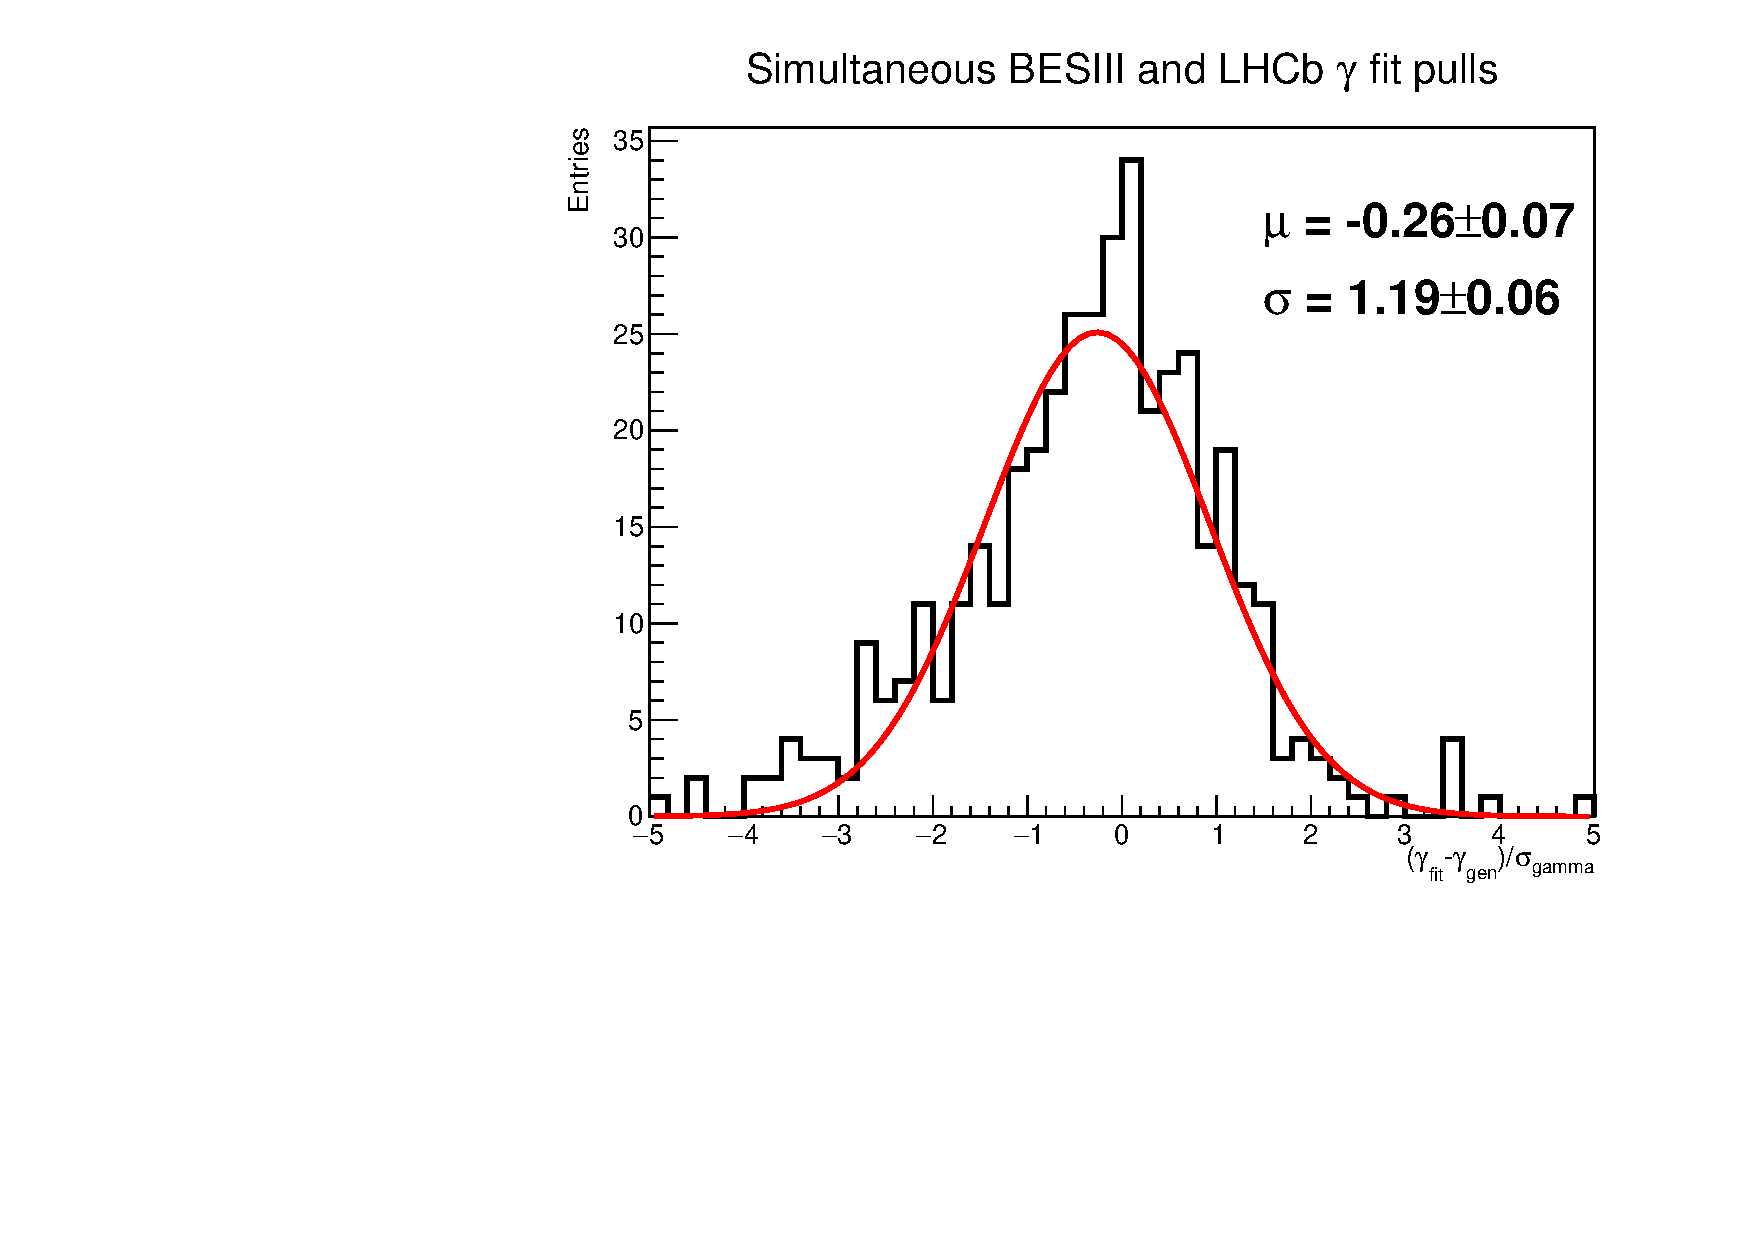
\includegraphics[width=0.6\textwidth]{Plots/Gamma_SimultaneousFit_pull.pdf}
  \end{figure}
  \begin{center}
    \large Stable fit with minimal bias and small undercoverage
  \end{center}
\end{frame}

\begin{frame}{Simultaneous fit of LHCb and BESIII bin yields}
  \begin{center}
    \large Study expected $\gamma$ uncertainty, after correcting for coverage:
  \end{center}
  \vspace{-0.3cm}
  \begin{figure}[htb]
    \centering
    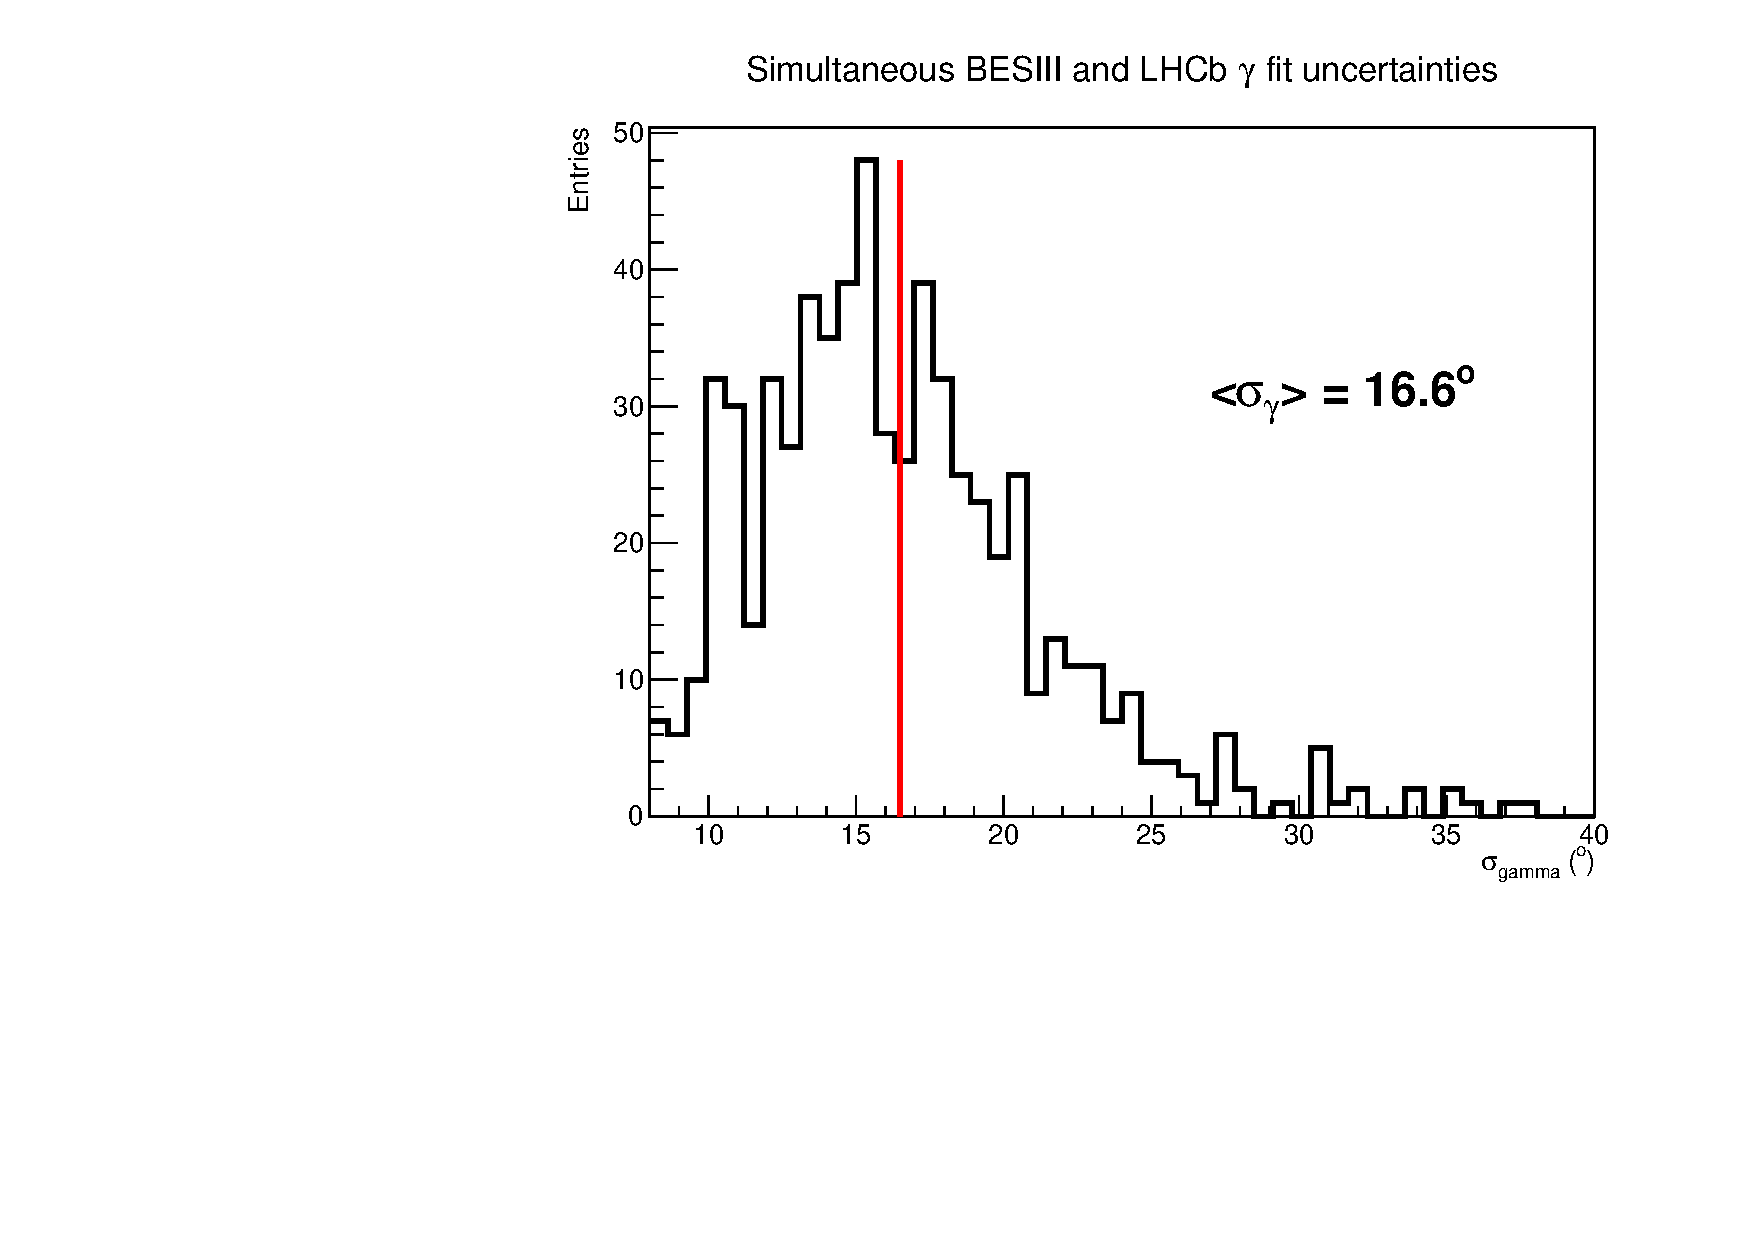
\includegraphics[width=0.5\textwidth]{Plots/Gamma_SimultaneousFit_err.pdf}
  \end{figure}
  \vspace{-0.4cm}
  {\large Conclusion from toy studies:}
  \vspace{-0.0cm}
  \begin{enumerate}
    \item{Well behaved fit, with expected sensitivity of $\sigma(\gamma) = 16.6^\circ$}
    \item{Only small corrections to bias and coverage required}
    \item{Will update $\gamma$ result once BESIII meausurement is released}
  \end{enumerate}
\end{frame}

\section{Importance of strong phases in charm mixing}

\begin{frame}{Charm mixing studies with multi-body decays}
  \begin{center}
    \Large The non-zero mass difference between $D^0$ and $\bar{D^0}$ was measured using the multi-body decay $D\to K_S^0\pi^+\pi^-$
  \end{center}
  \vspace{-0.2cm}
  \begin{figure}[htb]
    \centering
    \begin{subfigure}{0.5\textwidth}
      \vspace{-0.2cm}
      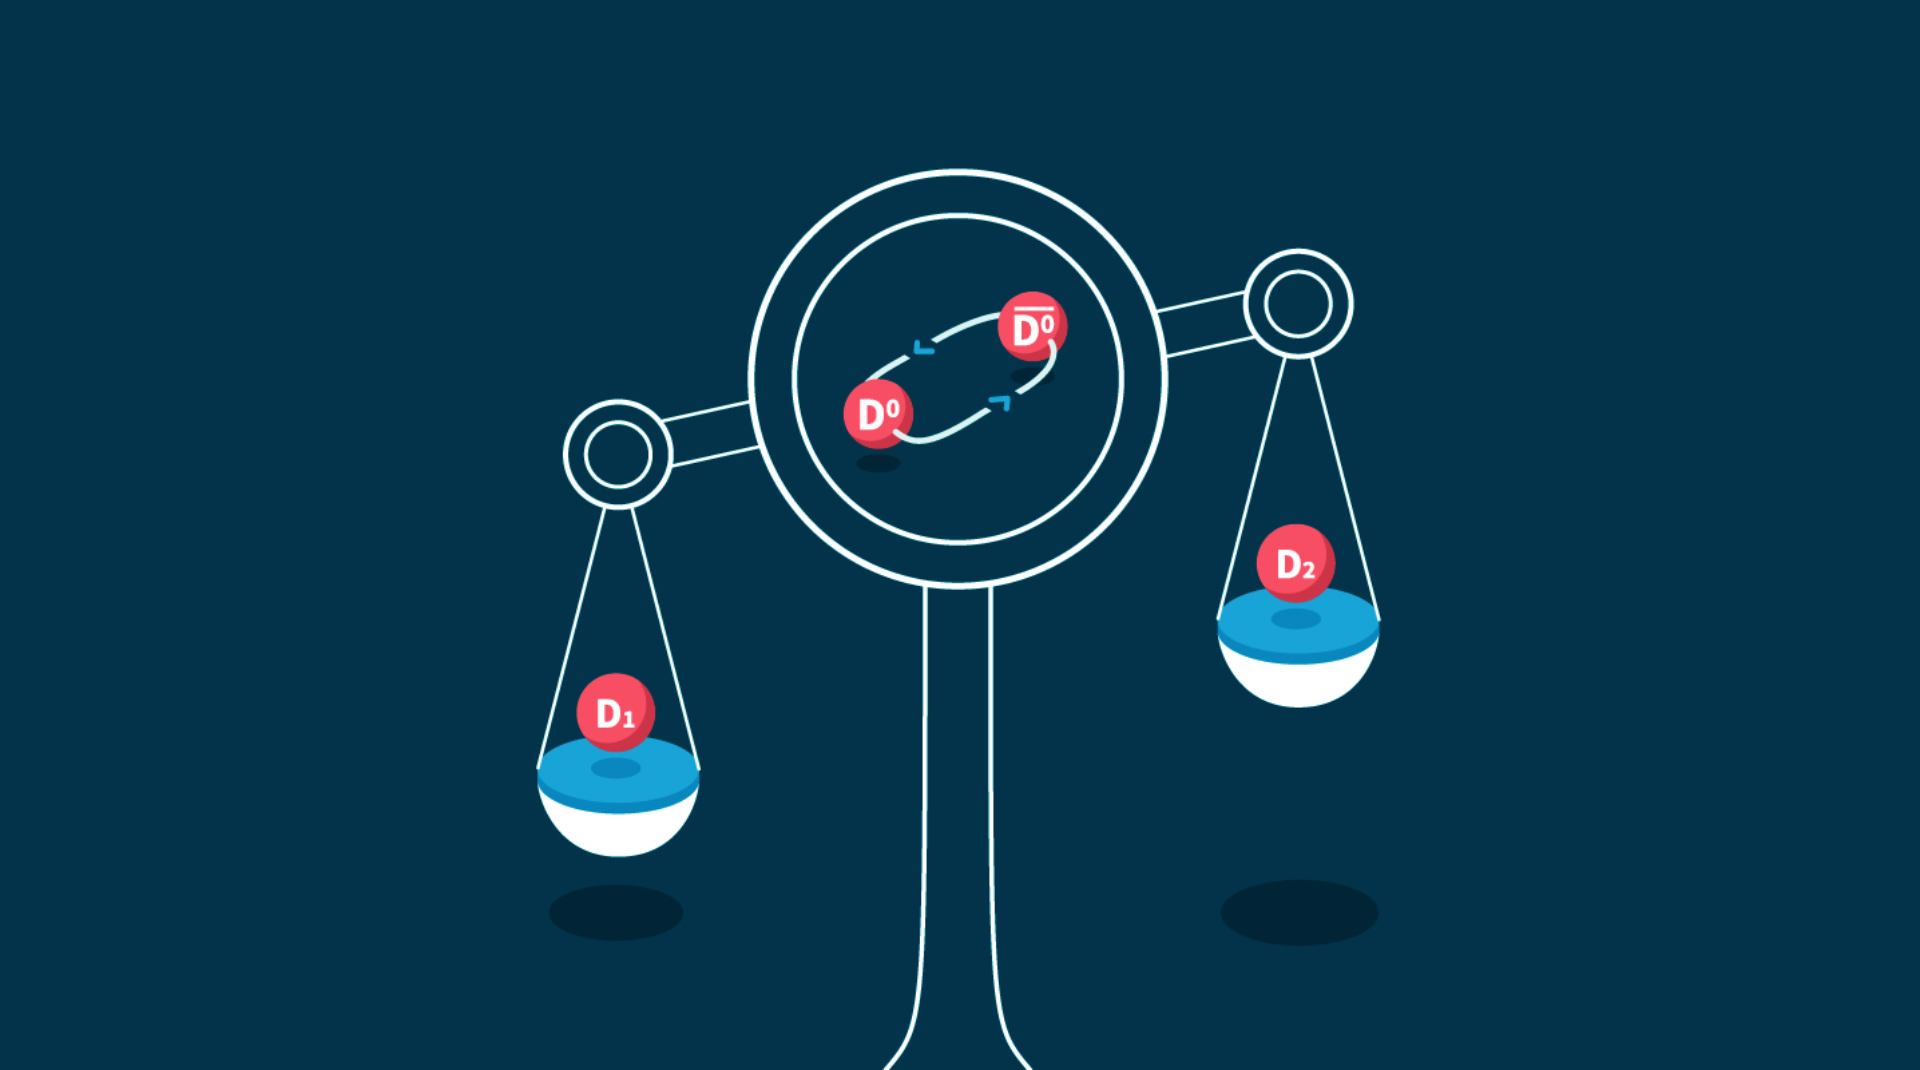
\includegraphics[width=1.0\textwidth]{Plots/CharmMassDifferenceIllustration.jpg}
    \end{subfigure}%
    \begin{subfigure}{0.5\textwidth}
      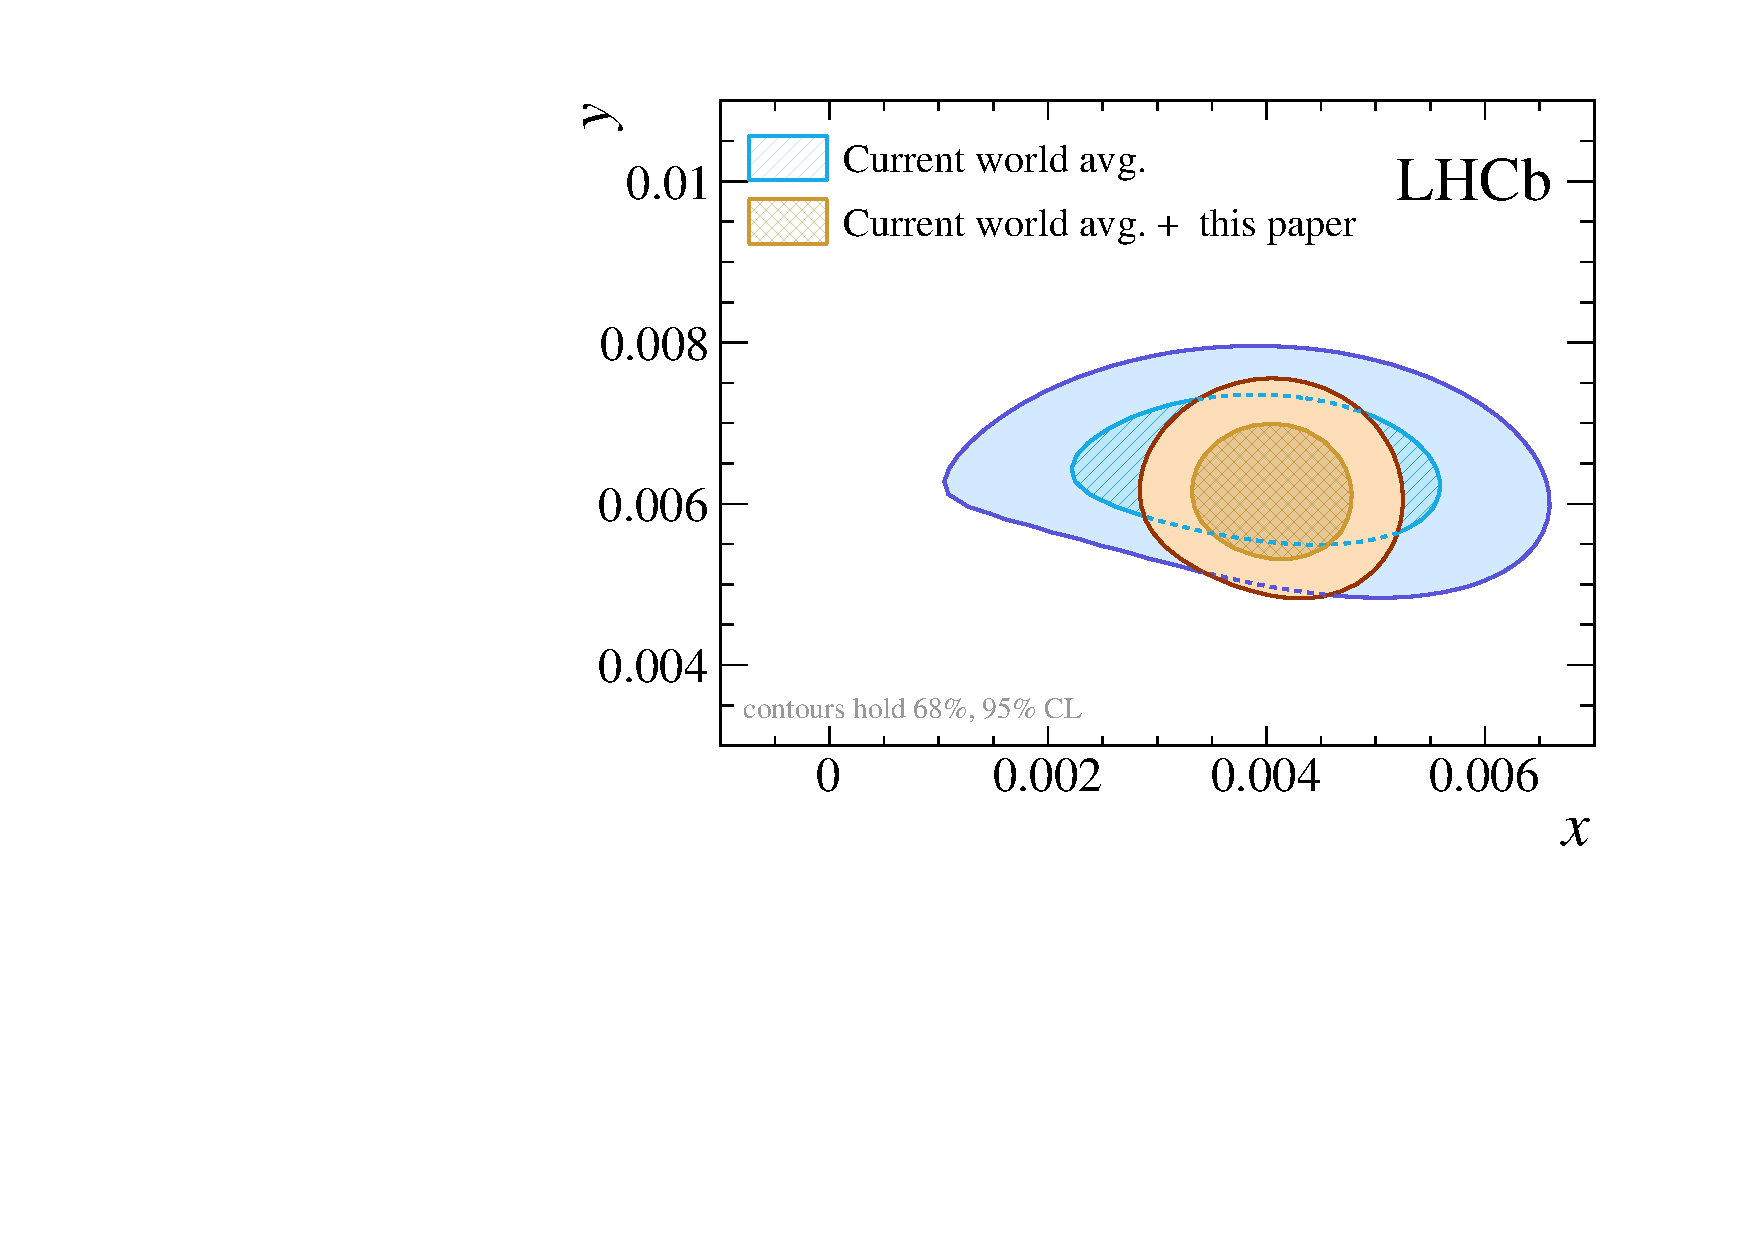
\includegraphics[width=1.0\textwidth]{Plots/KSpipi_xy_observation.pdf}
    \end{subfigure}
    \vspace{-0.5cm}
    \caption*{\tiny\href{https://journals.aps.org/prl/abstract/10.1103/PhysRevLett.127.111801}{Phys. Rev. Lett \textbf{127}, 111801 (2021)}}
  \end{figure}
  \vspace{-0.5cm}
  \begin{center}
    {\large Charm strong-phase differences were \underline{crucial} for this measurement!}
  \end{center}
\end{frame}

\begin{frame}{Charm mixing studies with multi-body decays}
  \begin{center}
    \Large Ongoing charm mixing study of $D\to h^+h^-\pi^+\pi^-$\\
    \normalsize by Jairus Tristan Patoc
  \end{center}
  \vspace{-0.2cm}
  \begin{columns}
    \begin{column}{0.5\textwidth}
      \vspace{-0.3cm}
      \begin{itemize}
        \setlength\itemsep{1.0em}
        \item{Prompt $D^{*+}\to D^0\pi^+$ sample}
        \item{Study $D^0\to h^+h^-\pi^+\pi^-$}
        \item{Run 2 ($\SI{6}{\per\femto\barn}$)}
        \item{Expected yields are}
        \begin{itemize}
          \item{$K^+K^-\pi^+\pi^-$: 4 million}
          \item{$\pi^+\pi^-\pi^+\pi^-$: 12 million}
        \end{itemize}
        \item{Current work:}
        \begin{enumerate}
          \item{Sensitivity and bias studies}
          \item{Optimised selection}
        \end{enumerate}
      \end{itemize}
    \end{column}
    \begin{column}{0.5\textwidth}
      \begin{figure}[htb]
        \centering
        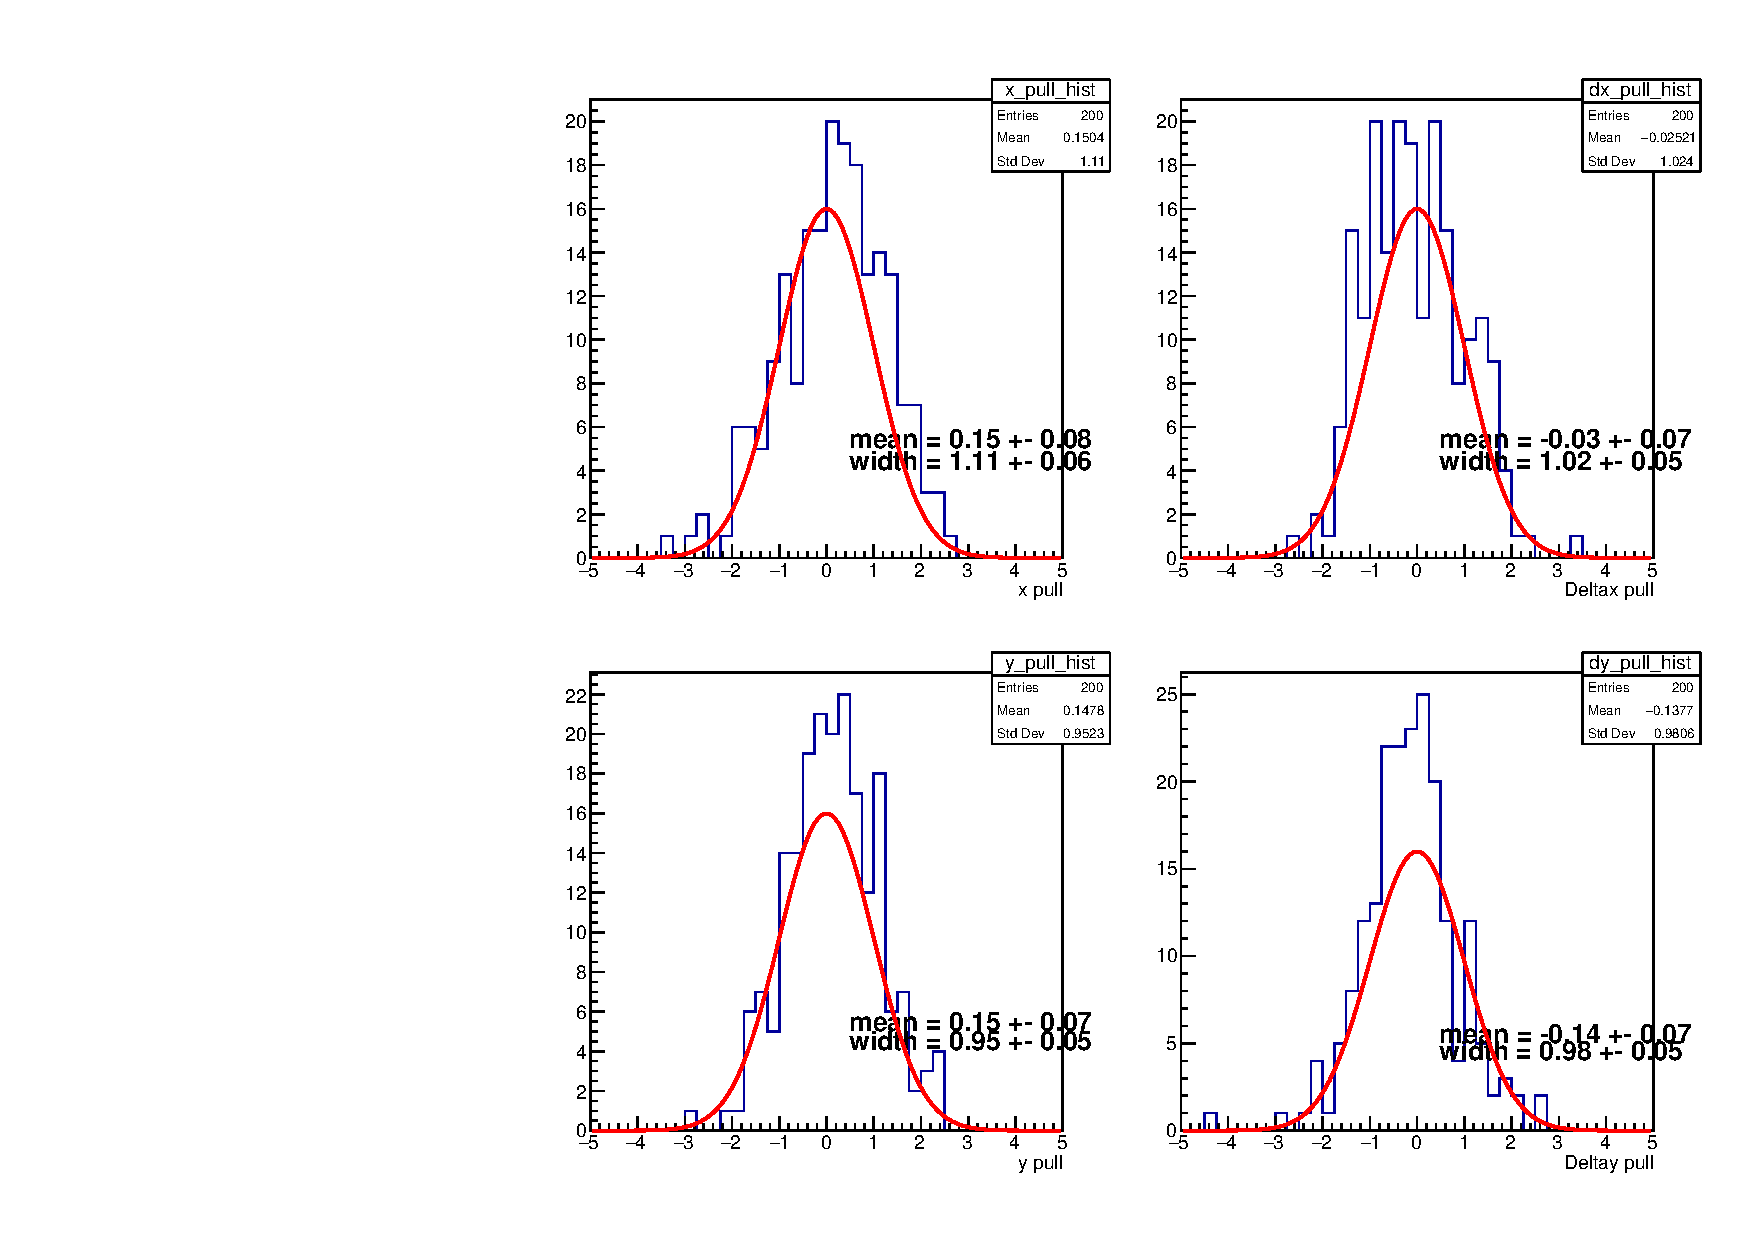
\includegraphics[width=1.0\textwidth]{Plots/PSbinned_pulls_CPtoy.pdf}
      \end{figure}
    \end{column}
  \end{columns}
\end{frame}

\begin{frame}{Charm mixing studies with multi-body decays}
  \begin{center}
    \large Mixing equations depend on $x$ and $y$, but also $c_i$ and $s_i$:
  \end{center}
  \vspace{-0.3cm}
  \begin{columns}
    \begin{column}{0.65\textwidth}
      \begin{block}{\centering 1. Charm mixing equations}
        $N_{D^0}(+i, \langle t\rangle_j) = K_{+i} - \sqrt{K_{+i}K_{-i}}\langle t\rangle_j(yc_i + xs_i)$ \\
        $N_{D^0}(-i, \langle t\rangle_j) = K_{-i} - \sqrt{K_{+i}K_{-i}}\langle t\rangle_j(yc_i - xs_i)$
      \end{block}
    \end{column}
  \end{columns}
  \begin{columns}
    \begin{column}{0.5\textwidth}
      \begin{enumerate}
        \setlength\itemsep{1.0em}
        \item{Fit the mixing equations}
        \item{Fit the ratio of mixing equations}
      \end{enumerate}
      \vspace{0.2cm}
      \begin{block}{\centering 2. Charm mixing ratio (bin-flip)}
        \begin{center}
          $R_i = \frac{K_{+i} - \sqrt{K_{+i}K_{-i}}\langle t\rangle_j(yc_i + xs_i)}{K_{-i} - \sqrt{K_{+i}K_{-i}}\langle t\rangle_j(yc_i - xs_i)}$
        \end{center}
      \end{block}
    \end{column}
    \begin{column}{0.5\textwidth}
      \begin{figure}[htb]
        \centering
        \begin{overpic}[percent,width=0.8\textwidth]{Plots/KSpipi_CharmMixingSlopes.pdf}
          \put(-133,60){\vector(1.0,-0.6){20}}
          \put(-133,86){\vector(1.0,1.0){30}}
        \end{overpic}
      \end{figure}
    \end{column}
  \end{columns}
\end{frame}

\begin{frame}{Charm mixing studies with multi-body decays}
  \begin{center}
    {\large Alternative strategy: Fix $x$ and $y$, and measure $c_i$ and $s_i$}
  \end{center}
  \vspace{-0.2cm}
  \begin{columns}
    \begin{column}{0.65\textwidth}
      \begin{block}{\centering 1. Charm mixing equations}
        $N_{D^0}(+i, \langle t\rangle_j) = K_{+i} - \sqrt{K_{+i}K_{-i}}\langle t\rangle_j(yc_i + xs_i)$ \\
        $N_{D^0}(-i, \langle t\rangle_j) = K_{-i} - \sqrt{K_{+i}K_{-i}}\langle t\rangle_j(yc_i - xs_i)$
      \end{block}
    \end{column}
  \end{columns}
  \vspace{0.1cm}
  \begin{itemize}
    \item{Two independent equations per bin, two observables per bin}
    \item{Similar statistical sensitivity to $c_i$ and $s_i$, in contrast to BESIII}
  \end{itemize}
  \vspace{-0.2cm}
  \begin{figure}[htb]
    \centering
    \begin{subfigure}{0.5\textwidth}
      \centering
      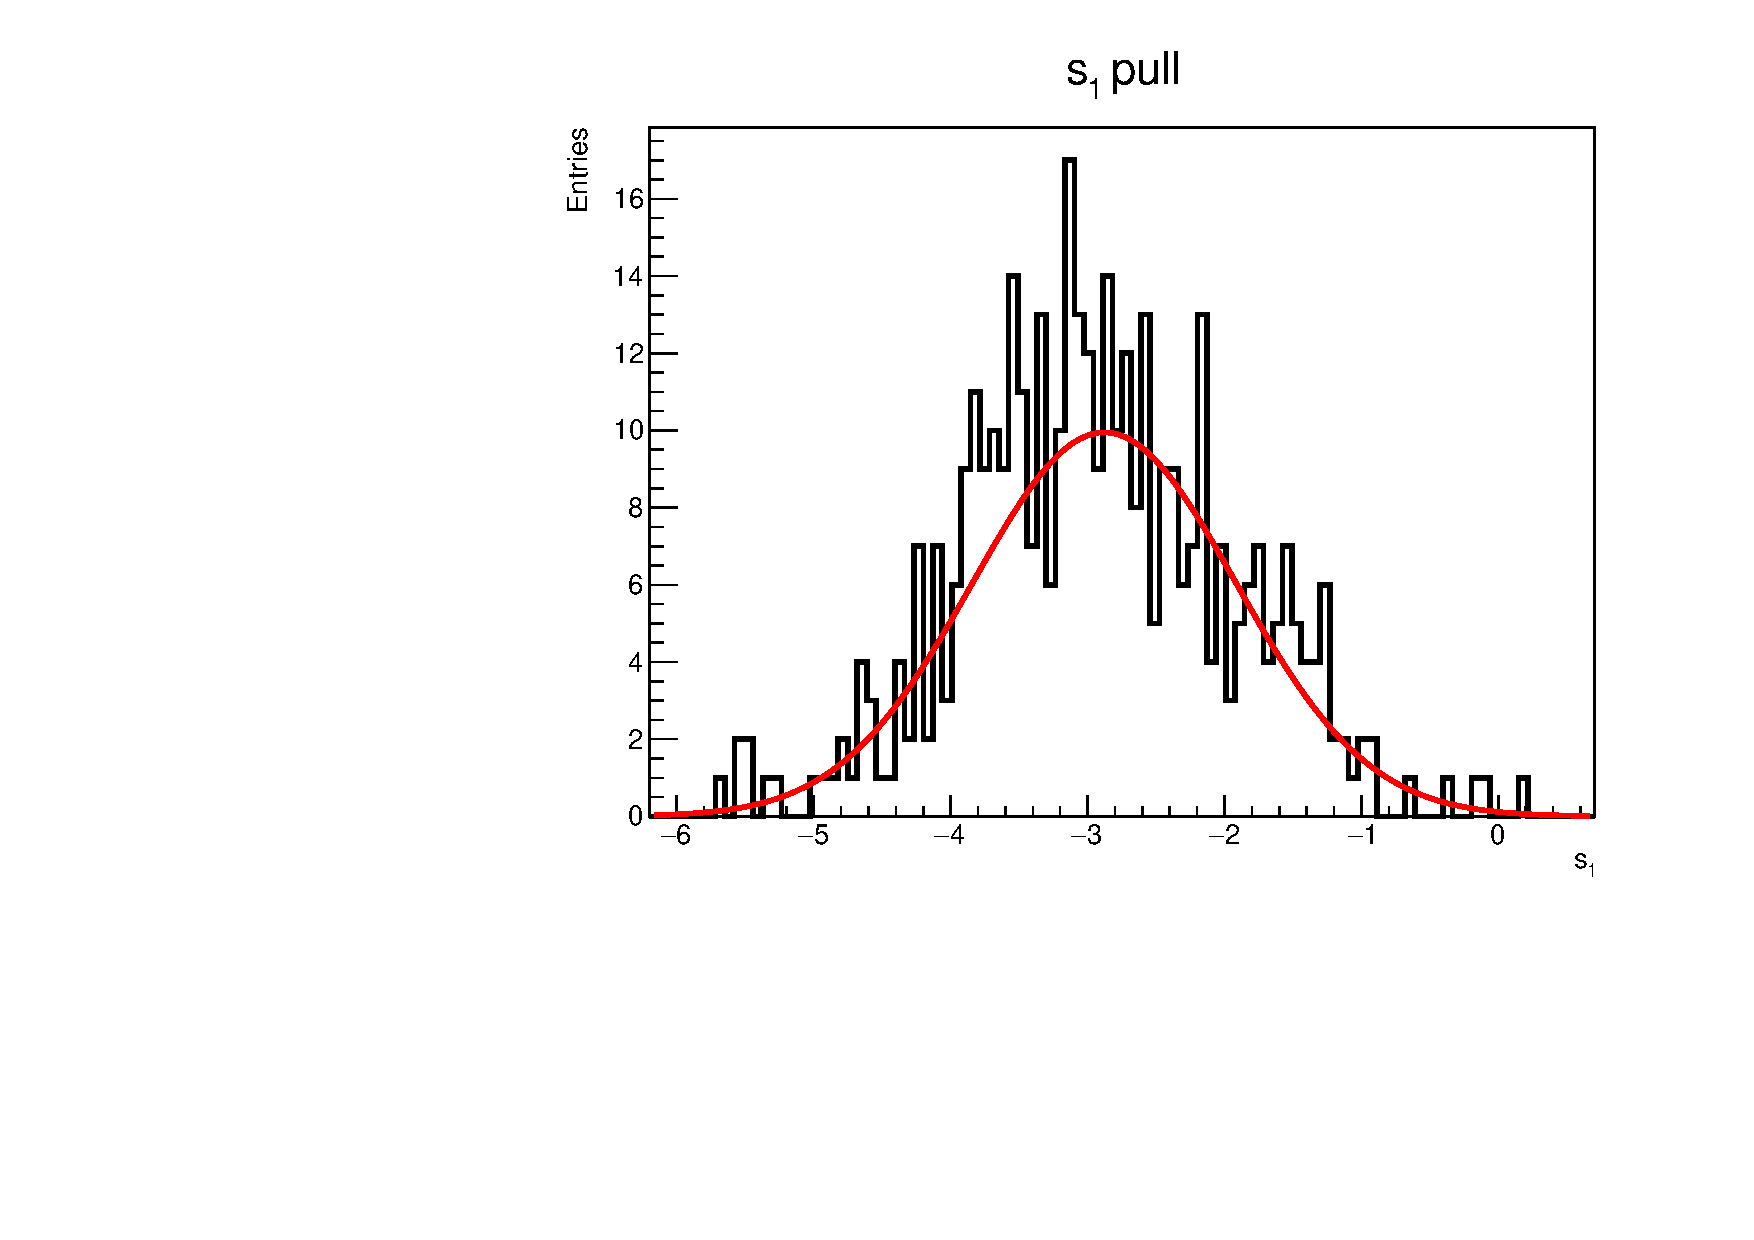
\includegraphics[width=0.8\textwidth]{Plots/s_1_pull_hist.pdf}
    \end{subfigure}%
    \begin{subfigure}{0.5\textwidth}
      \centering
      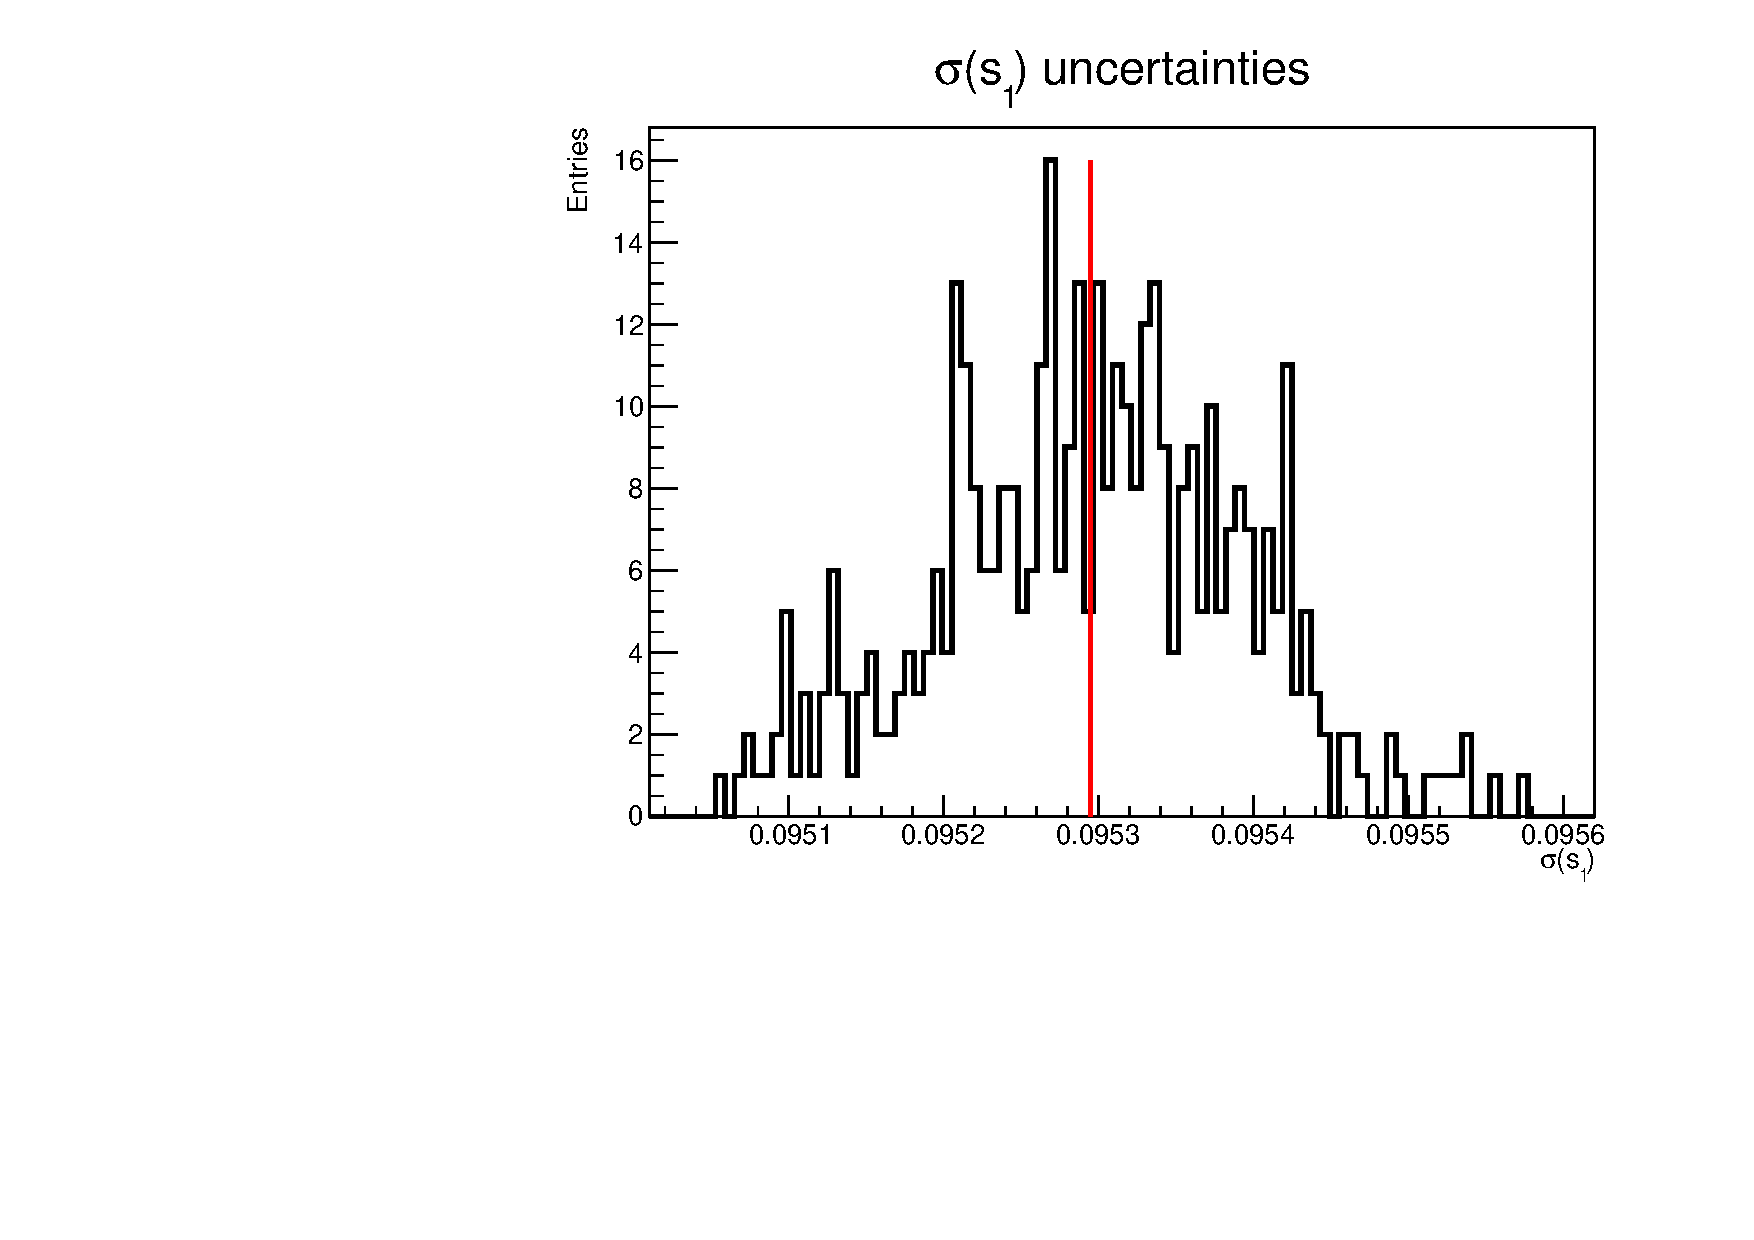
\includegraphics[width=0.8\textwidth]{Plots/s_1_err_hist.pdf}
    \end{subfigure}
    \vspace{-0.5cm}
  \end{figure}
\end{frame}

\begin{frame}{Charm mixing studies with multi-body decays}
  \begin{center}
    {\large Can also use bin-flip method to fit $s_i$, but $c_i$ must be fixed}
  \end{center}
  \vspace{-0.2cm}
  \begin{columns}
    \begin{column}{0.65\textwidth}
      \begin{block}{\centering 2. Charm mixing ratio (bin-flip)}
        \begin{center}
          $R_i = \frac{K_{+i} - \sqrt{K_{+i}K_{-i}}\langle t\rangle_j(yc_i + xs_i)}{K_{-i} - \sqrt{K_{+i}K_{-i}}\langle t\rangle_j(yc_i - xs_i)}$
        \end{center}
      \end{block}
    \end{column}
  \end{columns}
  \vspace{0.1cm}
  \begin{itemize}
    \item{Only one independent equation per bin}
    \item{Sensitivity found to be similar to fitting mixing equations directly}
  \end{itemize}
  \vspace{-0.2cm}
  \begin{figure}[htb]
    \centering
    \begin{subfigure}{0.5\textwidth}
      \centering
      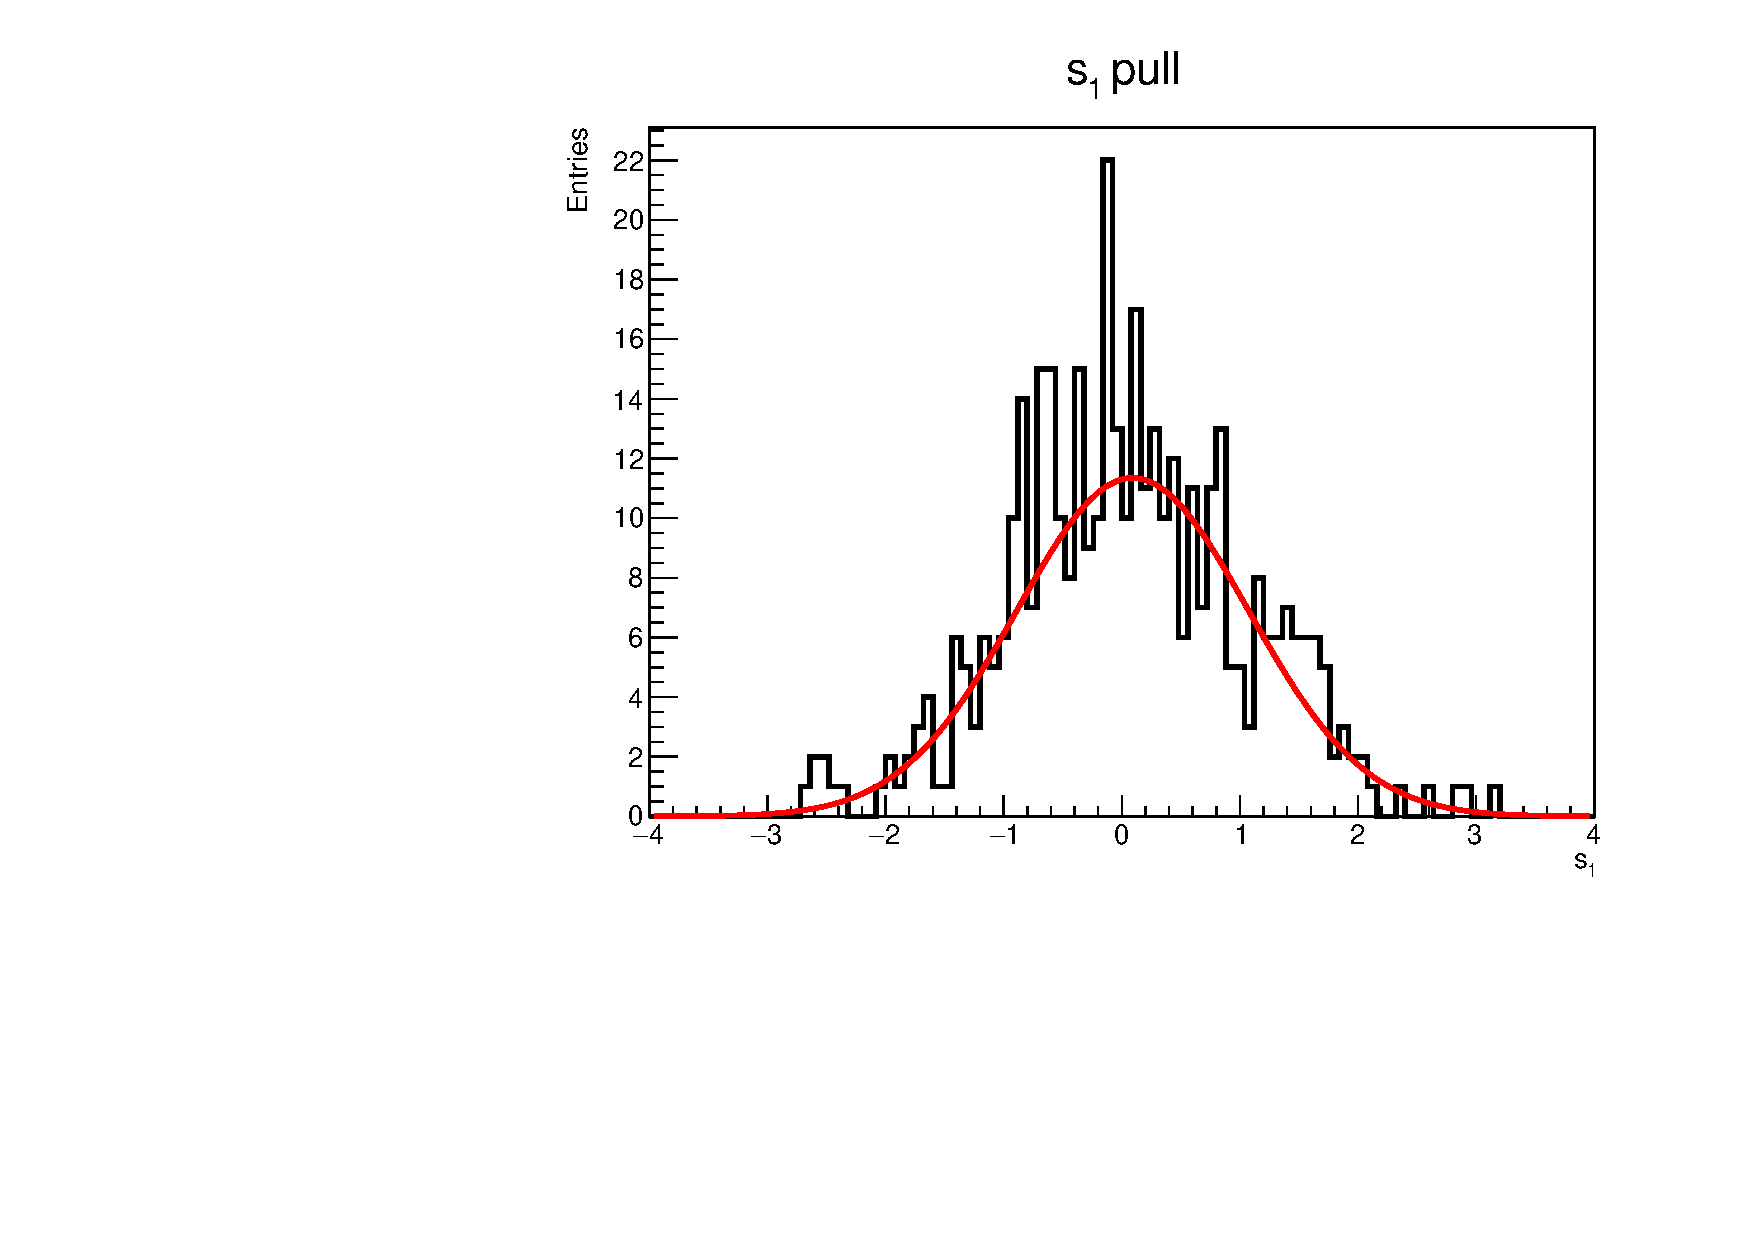
\includegraphics[width=0.8\textwidth]{Plots/s_1_pull_binflip_hist.pdf}
    \end{subfigure}%
    \begin{subfigure}{0.5\textwidth}
      \centering
      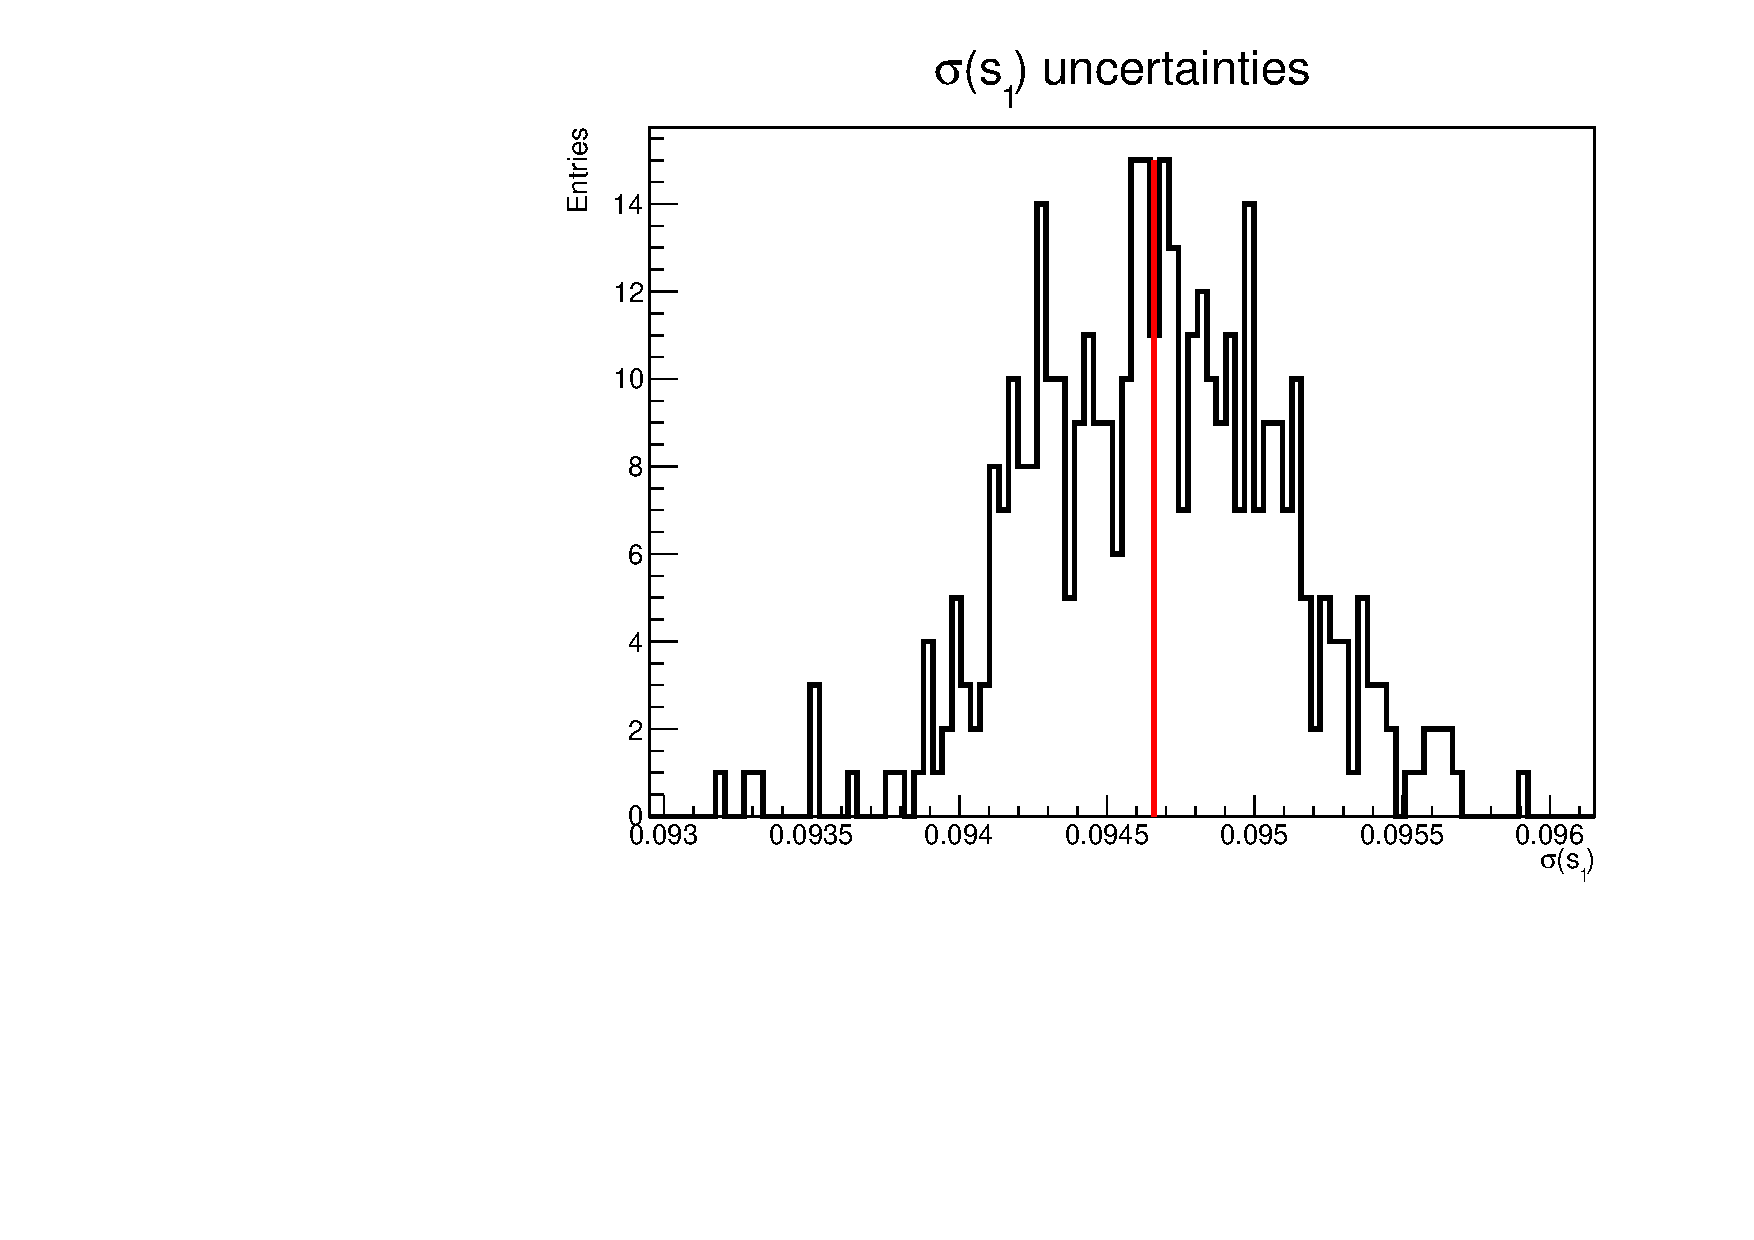
\includegraphics[width=0.8\textwidth]{Plots/s_1_err_binflip_hist.pdf}
    \end{subfigure}
    \vspace{-0.5cm}
  \end{figure}
\end{frame}

\begin{frame}{Charm mixing studies with multi-body decays}
  \begin{center}
    {\large Sensitivity to $c_i$: Similar between BESIII and charm mixing at LHCb}
  \end{center}
  \begin{figure}[htb]
    \centering
    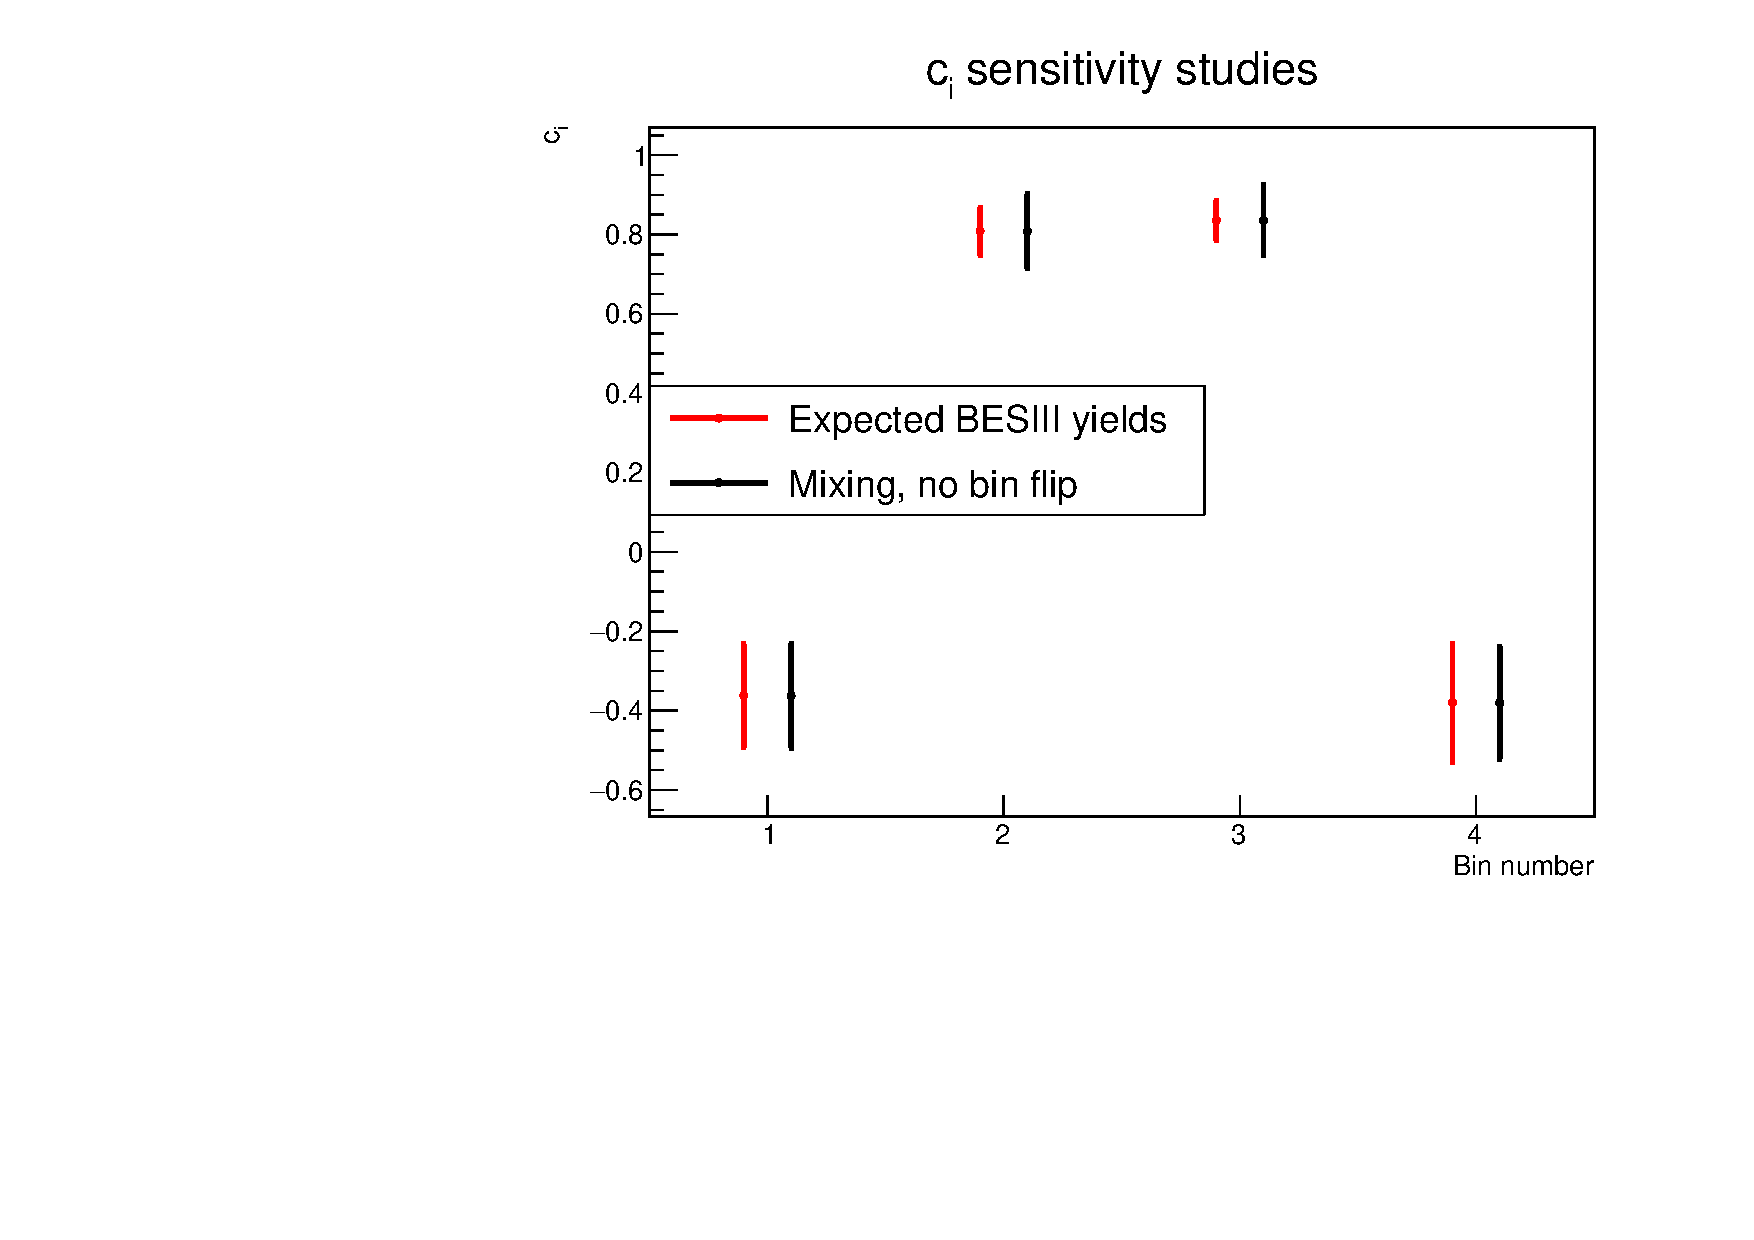
\includegraphics[width=0.7\textwidth]{Plots/ci_sensitivity.pdf}
  \end{figure}
  \vspace{-0.4cm}
  \begin{itemize}
    \item{BESIII yields equivalent to $\SI{8}{\per\femto\barn}$ of $\psi(3770)$}
    \item{4 million $D\to K^+K^-\pi^+\pi^-$ candidates in mixing analysis}
    \end{itemize}
\end{frame}

\begin{frame}{Charm mixing studies with multi-body decays}
  \begin{center}
    {\large Sensitivity to $s_i$: Significant improvements expected!}
  \end{center}
  \begin{figure}[htb]
    \centering
    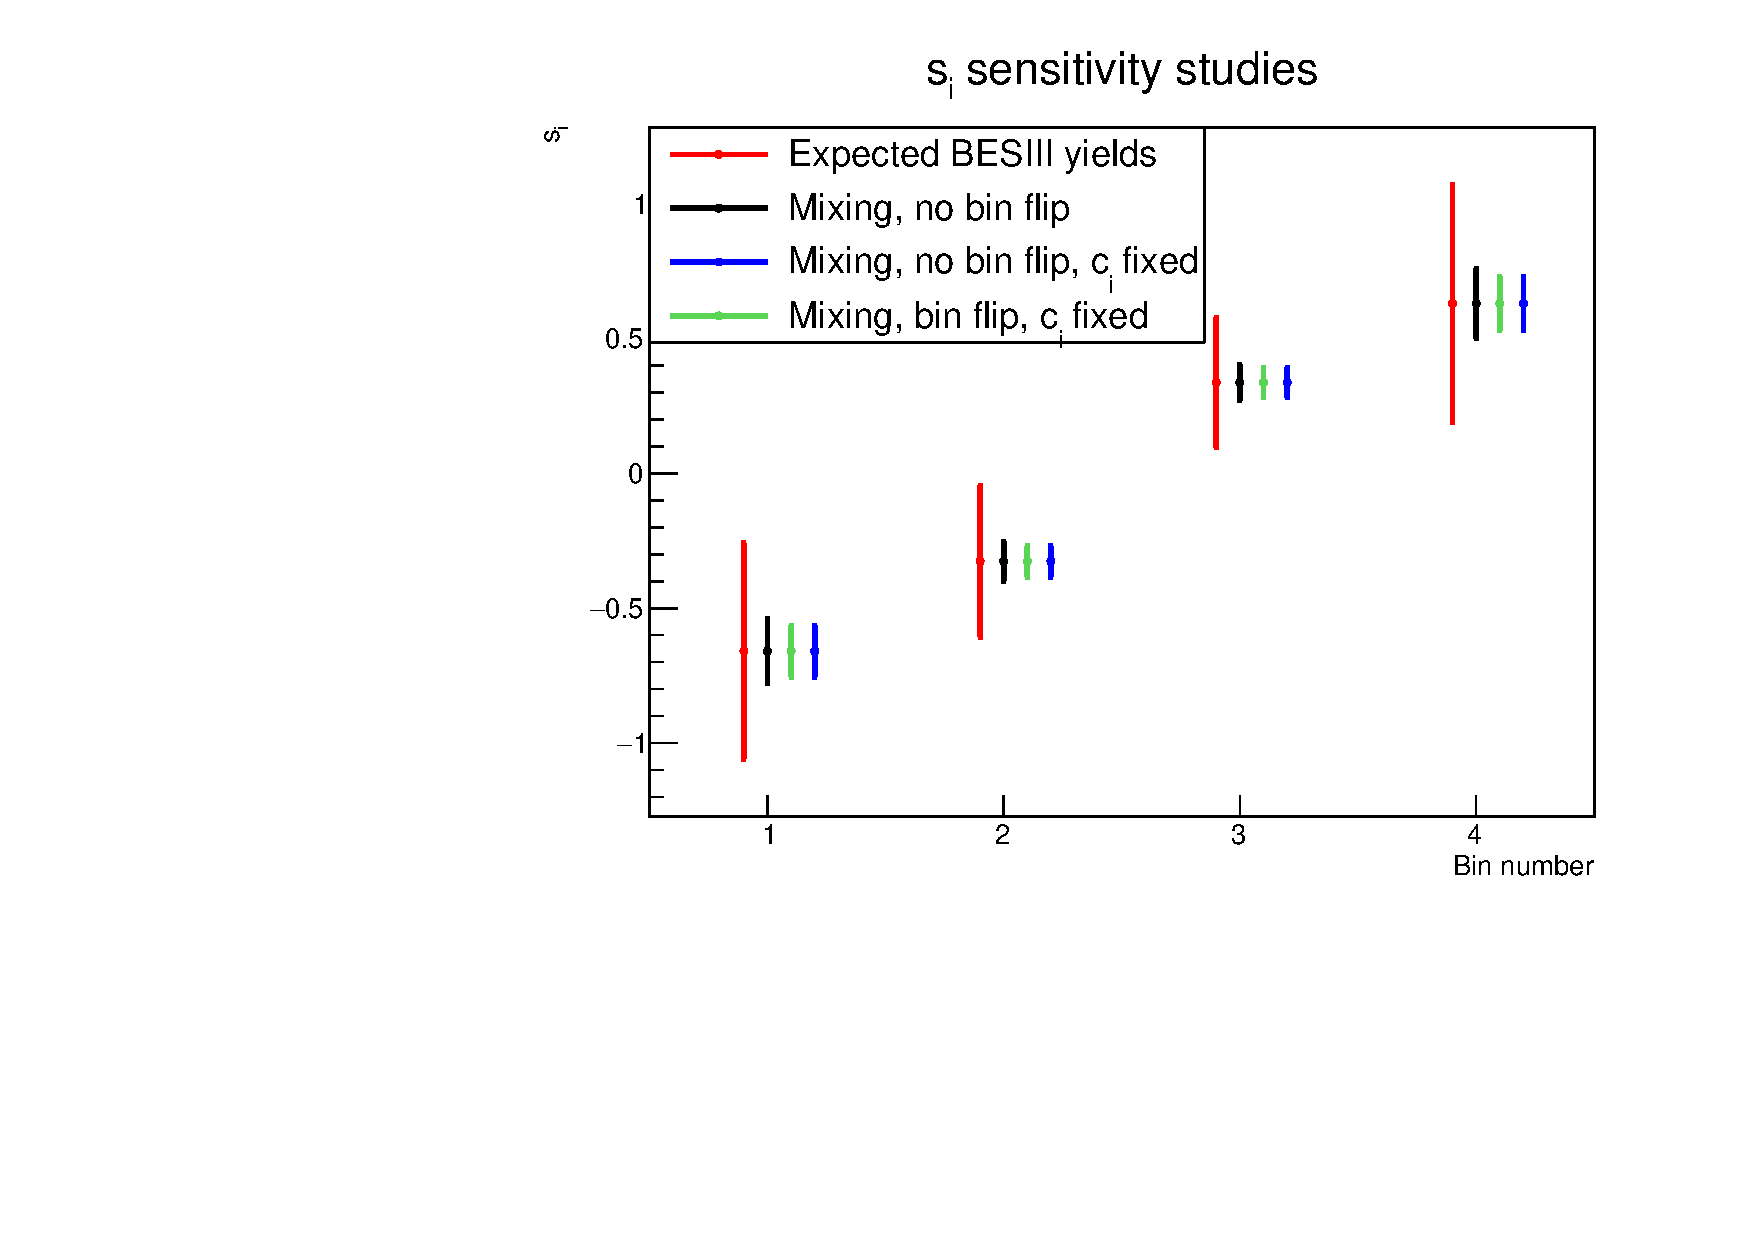
\includegraphics[width=0.7\textwidth]{Plots/si_sensitivity.pdf}
  \end{figure}
  \vspace{-0.4cm}
  \begin{itemize}
    \item{BESIII yields equivalent to $\SI{8}{\per\femto\barn}$ of $\psi(3770)$}
    \item{4 million $D\to K^+K^-\pi^+\pi^-$ candidates in mixing analysis}
  \end{itemize}
\end{frame}

\begin{frame}{Summary and future prospects}
  \vspace{0.3cm}
  {\Large Summary:}
  \vspace{0.5cm}
  \begin{enumerate}
    \setlength\itemsep{1.5em}
    \item{Measurement of $\gamma$ in $B^\pm\to[K^+K^-\pi^+\pi^-]_Dh^\pm$ is ready to be combined with \textbf{model-independent} strong-phase inputs}
    \item{BESIII strong-phase inputs can be further constrained using charm-mixing measurements at LHCb, and provide comparable sensitivity to $s_i$}
  \end{enumerate}
\end{frame}

\begin{frame}{Summary and future prospects}
  \vspace{0.3cm}
  {\Large Future prospects:}
  \vspace{0.5cm}
  \begin{enumerate}
    \setlength\itemsep{1.5em}
    \item{Measurement is still statistically limited, and will be significantly improved with LHCb Upgrade I}
    \item{Additional BESIII data and charm-mixing measurements from LHCb will bring strong-phase systematics down further}
    \item{Can extend this strategy to many more four-body modes}
    \begin{itemize}
      \item{Studies of $D\to\pi^+\pi^-\pi^+\pi^-$ show similar results}
    \end{itemize}
  \end{enumerate}
  \vspace{0.5cm}
  \begin{center}
    {\huge Thanks for your attention!}
  \end{center}
\end{frame}

\end{document}
